% I'm convinced by Peter's examples of min / max total mass being
% useful.  It will be interesting to see what types of calculations end
% up being most prevalent in our examples.  The interplay between total
% mass and the per-point mass function is interesting and seems like the
% sort of thing that mathematicians may have considered before.  I did
% some minor digging and Simplexes seem related:

% http://en.wikipedia.org/wiki/Simplex
% (also see http://en.wikipedia.org/wiki/Categorical_distribution)

% As a bonus, n-dimensional simplexes correspond directly to
% n-dimensional convex polyhedra.  One big difference between our
% distribution sets and simplexes is that we have bounds on the number
% of 0-valued points.

% Anyway, something to think about after we get this paper written.  I
% suspect there is a large space of possible abstractions for these
% distributions and it will be interesting to compare them (once we
% discover them :-)

\section{Belief revision via abstract interpretation}
\label{sec:absinterp}

\setlength{\arraycolsep}{0.1cm}
\newcommand{\ajoin}[0]{\bigsqcup}

% We could implement the belief semantics described in the previous
% section more-or-less directly, e.g., using an existing probabilistic
% language (such as IBAL~\cite{pfeffer07ibal} or Probabilistic
% Scheme~\cite{radul07probscheme}).  However, existing approaches use
% sampling to perform belief revisions, and for the examples of the sort
% given in Section~\ref{sec:examples}, the input space is too large for
% sampling to compute sound answers efficiently.  Therefore, we have
% developed a probabilistic semantics using abstract
% interpretation.

Consider how we might implement belief tracking and revision to
enforce the threshold security property given in
Definition~\ref{def:threshold}.  A natural choice would be to evaluate
queries using a probabilistic programming language with support for
conditioning, of which there are many \cite{pfeffer07ibal,
  radul07probscheme, park08sampling, goodman08church,
  kiselyov09embedded, claret12bayesian, milch05blog,
  borgstrom11measure}.  Such languages are largely
ineffective for use in ensuring security guarantees. Approximate
inference in these languages cannot ensure security guarantees, while
exact inference, due to its lack of abstraction facilities, can be too
inefficient when the state space is large.

%As more inputs are enumerated, a more complete view of the
%output distribution emerges.  Unfortunately, to get an accurate
%estimate of the revised distribution following an output observation,
%one must enumerate the entire input space, which could be quite large.
%If insufficient coverage is achieved, then the threshold check in
%Definition~\ref{def:threshold} could either be unsound or excessively
%conservative, depending in which direction an implementation errs.

We have developed a new means to perform probabilistic computation
based on abstract interpretation.  In this approach, execution time
depends on the complexity of the query rather than the size of the
input space.  In the next two sections, we present two abstract
domains.  This section presents the first, denoted $\ppolys$, where an
abstract element is a single \emph{probabilistic polyhedron}, which is
a convex polyhedron~\cite{CousotHalbwachs78-POPL} with information
about the probabilities of its points. 

Because using a single polyhedron will accumulate imprecision after
multiple queries, in our implementation we actually use a different
domain, denoted $ \ppowers $, for which an abstract element consists
of a set of at most $n$ probabilistic polyhedra (whose construction is
inspired by powersets of polyhedra
\cite{bagnara06powerset,Popeea06inferringdisjunctive}).  This domain,
described in the next section, allows us to retain precision at the
cost of increased execution time.  By adjusting $n$, the user can
trade off efficiency and precision. An important element of our
approach is the ability to soundly evaluate the knowledge-threshold
policies, even under approximate inference.

\subsection{Polyhedra} \label{sec:polyhedra}

We first review \emph{convex polyhedra}, a common technique for representing sets of program states.  We use the meta-variables $\ineq, \ineq_1, \ineq_2$, etc. to denote linear inequalities.  We write $\fv\ineq$ to be the set of variables occurring in
$\ineq$; we also extend this to sets, writing $\fv{\{\ineq_1,\ldots,\ineq_n\}}$ for $\fv{\ineq_1} \cup \ldots \cup \fv{\ineq_n}$.

\begin{definition}
  A \emph{convex polyhedron} $\poly = (\cons, V)$ is a set of linear inequalities
  $\cons = \{\ineq_1,\ldots,\ineq_m\}$, interpreted conjunctively,
  over dimensions $ V $.  We write
  $\cp$ for the set of all convex polyhedra.   A polyhedron $\poly$
  represents a set of states, denoted $\pconc{\poly}$, as follows, where $\sigma \models \ineq$ indicates that the state $\sigma$ satisfies the inequality $\ineq$.
\[\pconc{\paren{\cons,V}} \defeq \{\sigma \given \fv{\sigma} =
V,\; \forall \ineq \in \cons.\ \sigma \models \ineq\}\]

Naturally we require that $\fv{\{\ineq_1,\ldots,\ineq_n\}} \subseteq V
$. We write $ \fv{\paren{\cons, V}} $ to denote the set of variables $
V $ of a polyhedron.

\end{definition}

% Figure \ref{fig:polyhedra} gives an example of a
% polyhedron $\poly$ and the set of states $\pconc{\poly}$.
Given a state $\sigma$ and an ordering on the variables in $\fv{\sigma}$, we can view $\sigma$ as a point in
an $N$-dimensional space, where $N = \setsize{\fv{\sigma}}$.  The set $\pconc{\poly}$ can then be viewed as the integer-valued lattice points in an $N$-dimensional polyhedron.
Due to this correspondence, we use the words \textit{point} and
\textit{state} interchangeably.  We will sometimes write linear equalities $x = f(\vec{y})$ as an abbreviation for the pair of inequalities $x \leq f(\vec{y})$ and $x \geq f(\vec{y})$.
% \todo{TODO: draw this picture.}

\newcommand{\myitem}{~\\ \noindent $\bullet$ }
Let $ \poly = (\cons, V) $. Convex polyhedra support the following
operations.
\begin{itemize}
%   We
% write $\setsize{S}$ to represent the cardinality of the set $S$.
\item Polyhedron size, or $ \psize{\poly} $, is the number of
   integer points in the polyhedron, i.e., $\setsize{\pconc{\poly}}$.
   We will always consider bounded polyhedra when determining their
   size, ensuring that $\psize{\poly}$ is finite.
\item (Logical) expression evaluation, $\abseeval{\bexp}{\poly}$ returns a
   convex polyhedron containing at least the points in $\poly$ that satisfy
$\bexp$. Note that $ B $ may or may not have disjuncts.
\item Expression count, $\absecount{\bexp}{\poly}$ returns an upper bound
 on the number of integer points in $\poly$ that satisfy $\bexp$. Note
 that this may be more precise than $\psize{\abseeval{\bexp}{\poly}}$
 if $ B $ has disjuncts.
% \sbmcomment{Because these are abstract operations (and may be approximate).
% $\absecount{\bexp}{\poly} \leq \psize{\abseeval{\bexp}{\poly}}$ but they may
% not be equal (and will not be for polyhedra).  Image the condition $\neg(x = 0)$.
% If $\poly$ is $-5 \leq x \leq 5$ then $\abseeval{\bexp}{\poly}$ is $-5 \leq x \leq 5$,
% which has 11 points, while $\absecount{\bexp}{\poly}$ could return $10$.
% Our implementation of $\absecount{\bexp}{\poly}$ proceeds by introducing some
% disjunction (thus retaining more precision) before doing the counting.  So it would count
% the points in the two polyhedra given by $-5 \leq x \leq -1$ and $1 \leq x \leq 5$.
% (These disjuncts can then either be thrown away or kept, depending on whether we are
% in the single polyhedron domain or the powerset domain.)
% While we implement a rather roundabout way of computing points consistent with $\bexp$
% (introduce disjunctions, take intersections, count),
% it's possible that a more direct method could be devised.  In any case, given the fact
% that considering this operation separately can improve precision, it seemed worth keeping
% it separate.  It also corresponds nicely with $\abseeval{\bexp}{\poly}$ (which is
% more precise than its ``naive'' implementation as $\poly \pmeet \alpha(\bexp)$, where
% $\alpha$ is the abstraction function returning the smallest convex polyhedron containing $\bexp$).
% }
 \item Meet, $ \pa \pmeet \pb $ is the convex
 polyhedron containing exactly the set of points in the intersection of
 $\pconc{\pa}, \pconc{\pb}$.
\item Join, $\pa \pjoin \pb$ is the smallest convex
 polyhedron containing both $\gamma(\pa)$ and $\gamma(\pb)$.
\item Comparison, $\pa \pord \pb$ is a partial order whereby $\pa \pord \pb$ if and only if $\pconc{\pa} \subseteq \pconc{\pb}$.
\item Affine transform, $\poly \bparen{x \ra \aexp}$, where $x
  \in \fv{\poly} $, computes an affine transformation of $ \poly $.  This scales
  the dimension corresponding to $x$ by the coefficient of $x$ in
  $\aexp$ and shifts the polyhedron.  For example, $\paren{\{x \leq y, y =
  2z\}, V} \bparen{y \ra z + y}$ evaluates to $\paren{\{x \leq y - z, y - z =
  2z\}, V}$.
\item Forget, $\forget{x}{\poly}$, projects away $x$.  That is,
  $\forget{x}{\poly} = \pi_{\fv{\poly}-\{x\}}(\poly)$, where
  $\pi_V(\poly)$ is a polyhedron $\poly'$ such that $\pconc{\poly'} =
  \{ \sigma \given \tau \in \pconc{\poly} \wedge \sigma =
  \project{\tau}{V} \}$.  So $\poly' = \forget{x}{\poly}$ implies
  $x \not\in fv(\poly')$. The projection of $ \getpoly{} $ to
  variables $ V $, written $ \project{\getpoly{}}{V}$ is defined as
  the forgetting of all the dimensions of $ \getpoly{} $ other than $
  V $.
%\item{} Add dimensions, $ \newdim{V'}{\poly} $ is the polyhedron with
%  additional dimensions $ V' $ that are disjoint from $ \fv{\poly} $. Thus $
%  \fv{\newdim{V'}{\poly}} = \fv{\poly} \cup V' $ with the dimensions $ V'
%  $ unconstrained. If $ V' = \set{x_1, \cdots, x_m} $ then $
%  \pconc{\newdim{V'}{C}} = \set{\sigma \cup \set{x_i = n_i}_{i=1}^{m}
%    \given \sigma \in \pconc{C}, n_i \in \Integer} $.  We write $
%  \sigma \cup \set{x = n} $ to denote a state $ \sigma $ with an
%  additional assignment of $ x $ to value $ n $. 
\item{} Linear partition $\partn{\getpoly{A}}{\getpoly{B}}$  
  of two (possibly overlapping) polyhedra $ \getpoly{A} $, $
  \getpoly{B} $ is a set of equivalent disjoint polyhedra $
  \set{\getpoly{i}}_{i=1}^{n} $. That is, $ \cup_i \pconc{\getpoly{i}}
  = \pconc{\getpoly{A}} \cup \pconc{\getpoly{B}} $ and $
  \pconc{\getpoly{i}} \cap \pconc{\getpoly{j}} = \emptyset $ for $ i
  \neq j $.  When $\getpoly{A}$ and $\getpoly{B}$ do not overlap then
  $\partn{\getpoly{A}}{\getpoly{B}} = \set{\getpoly{A},\getpoly{B}}$.
\end{itemize}

We write $\isempty{\poly}$ \emph{iff} $\pconc{\poly} = \emptyset$.

\subsection{Probabilistic Polyhedra}

We take this standard representation of sets of program states and
extend it to a representation for sets of distributions over program
states.  We define \emph{probabilistic polyhedra}, the core element of
our abstract domain, as follows.

\begin{definition} \label{def:ppoly}
A \emph{probabilistic polyhedron} $\pp{}$ is a tuple
$(\getpoly{},\smin{},$ $\smax{}, \pmin{},$ $\pmax{}, \mmin{},$ $\mmax{})$.  
We write $\ppolys$ for the set of probabilistic polyhedra.  The
quantities $\smin{}$ and $ \smax{}$ are lower and upper bounds on 
the number of support points in the polyhedron $\getpoly{}$.  The quantities
$\pmin{} $ and $ \pmax{} $ are lower and upper bounds on the
probability mass \emph{per support point}.  The $ \mmin{} $ and $
\mmax{} $ components give bounds on the total probability mass.  
Thus $\pp{}$ represents the \emph{set} of distributions
$\ppconc{\pp{}}$ defined below. 
\[
\ppconc{\pp{}} \defeq
\begin{aligned}[t]
\{\delta \given {} & \nzset{\delta} \subseteq \pconc{\getpoly{}} \wedge {} \\
  & \smin{} \leq \setsize{\nzset{\delta}} \leq \smax{} \wedge {} \\
  & \mmin{} \leq \pmass{\delta} \leq \mmax{} \wedge \\
  & \forall \sigma \in \nzset{\delta}.\ \pmin{} \leq \delta(\sigma) \leq \pmax{}\}
\end{aligned}
\]

We will write $ \fv{\pp{}} \defeq \fv{\poly} $ to denote the set of variables
used in the probabilistic polyhedron. 

\end{definition}
% Recall that $\pmass{\delta}$ gives the mass of distribution $\delta$,
% which is the sum of the probabilities ascribed to states by $\delta$. 
Note the set $\ppconc{\pp{}}$ is a singleton exactly when $\smin{} =
\smax{} = \psize{\getpoly{}}$ and $\pmin{} = \pmax{}$, and $\mmin{} =
\mmax{}$.  In such a case $\ppconc{\pp{}}$ contains only the uniform
distribution where each state in $\pconc{\getpoly{}}$ has probability
$\pmin{}$. In general, however, the concretization of a probabilistic
polyhedron will have an infinite number of distributions. For example,
the pair of probabilistic polyhedra in \sref{sec:overview},
Equation~\ref{eq-nonuniform} admits an infinite set of distributions,
with per-point probabilities varied somewhere in the range $ \pmin{1}
$ and $ \pmax{1} $. The representation of the non-uniform distribution
in that example is thus approximate, but the security policy can still
be checked via the $ \pmax{1} $ (and $ \mmax{2} $) properties of the
probabilistic polyhedron.

Distributions represented by a probabilistic polyhedron
are not necessarily normalized (as was true in
Section~\ref{sec:clarkson-semantics}).  In general, there is a
relationship between $\pmin{}, \smin{}, $ and $\mmin{}$, in that
$\mmin{} \geq \pmin{} \cdot \smin{}$ (and $\mmax{} \leq \pmax{} \cdot
\smax{}$), and the combination of the three can yield more information
than any two in isolation.

Our convention will be to use $\getpoly{1}$, $\smin{1}$, $\smax{1}$,
etc. for the components associated with probabilistic polyhedron
$\pp{1}$ and to use subscripts to name different probabilistic
polyhedra.

\myparagraph{Ordering}
Distributions are ordered point-wise~\cite{clarkson09quantifying}.
That is, $\delta_1 \leq \delta_2$ if and only if $\forall
\sigma.\ \delta_1(\sigma) \leq \delta_2(\sigma)$.  For
our abstract domain, we say that $\pp{1} \ppord \pp{2}$ if and only if
$\forall \delta_1 \in \ppconc{\pp{1}}.\ \exists \delta_2 \in
\ppconc{\pp{2}}.\ \delta_1 \leq \delta_2$.  Testing $\pp{1} \ppord
\pp{2}$ mechanically is non-trivial, but is unnecessary in our
semantics.  Rather, we need to test whether a distribution
represents only the zero distribution $\distzero \defeq \lambda
\sigma. 0$ in order to see that a fixed point for evaluating
$\abspevalp{\swhile{\bexp}{\stmt}}{\pp{}}$ has been reached.
Intuitively, no further iterations of the loop need to be considered
once the probability mass flowing into the $n^\text{th}$ iteration is
zero. This condition can be detected as follows:
% \vspace*{-0.9em}
% \begin{small}
\[
\begin{array}{l}
\iszero{\pp{}} \defeq \\
\qquad \paren{\smin{} = \smax{} = 0 \wedge \mmin{} = 0 \leq \mmax{}} \\
\quad \vee\; \paren{\mmin{} = \mmax{} = 0 \wedge \smin{} = 0 \leq \smax{}} \\
\quad \vee\; \paren{\isempty{\poly} \wedge \smin{} = 0 \leq \smax{} \wedge
\mmin{} = 0 \leq \mmax{}} \\
\quad \vee\; \paren{\pmin{} = \pmax{} = 0 \wedge \smin{} = 0 \leq \smax{} \wedge
\mmin{} = 0 \leq \mmax{}} \\
\end{array}
\]
% \end{small}
If $ \iszero{\pp{}} $ holds, it is the case that $ \ppconc{\pp{}} =
\set{\distzero} $.  This definition distinguishes $\ppconc{\pp{}} =
\emptyset $ (if $ \pp{} $ has inconsistent constraints) from 
$\ppconc{\pp{}} = \set{\distzero} $.  Note that having a more
conservative definition of $\iszero{\pp{}}$ (which holds for fewer
probabilistic polyhedra $\pp{}$) would simply mean our analysis would
terminate less often than it could, with no effect on
security.
%If $ \iszero{\pp{}} $ holds, it is the case that $ \ppconc{\pp{}} =
%\set{\distzero} $.  This definition has been carefully crafted to
%avoid treating a polyhedron with inconsistent constraints (which could
%arise when abstractly interpreting dead code) as being equivalent to
%$\set{\distzero}$; i.e., we must distinguish when $\ppconc{\pp{}} =
%\emptyset $ (arising from inconsistent constraints) from when
%$\ppconc{\pp{}} = \set{\distzero} $.  Note that having a more
%conservative definition of $\iszero{\pp{}}$ (which holds for fewer
%probabilistic polyhedra $\pp{}$) would simply mean our analysis would
%terminate less often than it could, with no effect on
%security. 

Following standard abstract interpretation terminology, we will refer
to $\powerset{\dists}$ (sets of distributions) as the \textit{concrete
  domain}, $\ppolys$ as the \textit{abstract domain}, and $\ppconcfun
: \ppolys \rightarrow \powerset{\dists}$ as the \textit{concretization
  function} for $\ppolys$.


\subsection{Abstract Semantics for $\ppolys$}

To support execution in the abstract domain just defined, we need
to provide abstract implementations of the basic operations of assignment,
conditioning, addition, and scaling used in the concrete semantics given in
Figure \ref{fig-sem-nondet2-core}.  We will overload notation and use the
same syntax for the abstract operators as we did for the concrete operators.

As we present each operation, we will also state the associated
soundness theorem which shows that the abstract operation is an
over-approximation of the concrete operation. Proofs are given in a
separate technical report~\cite{TR}.

The abstract program semantics is then exactly the semantics from
Figure \ref{fig-sem-nondet2-core}, but making use of the abstract
operations defined here, rather than the operations on distributions
defined in Section \ref{sec:clarkson-semantics}.  We will write
$\abspevalp{S}{\pp{}}$ to denote the result of executing $S$ using the
abstract semantics.  The main soundness theorem we obtain is the
following.
\begin{theorem}
\label{thm:pp:soundness}
For all $\pp{}, \delta$, if $ \delta \in \ppconc{\pp{}} $ and
$ \abspevalp{S}{\pp{}} $ terminates, then $ \pevalp{S}{\delta} $ terminates and $
\pevalp{S}{\delta} \in \ppconc{\abspevalp{S}{\pp{}}} $.
\end{theorem}

When we say $ \pevalp{S}{\delta} $ terminates (or $
\abspevalp{S}{\pp{}} $ terminates) we mean that only a finite number
of loop iterations are required to interpret the statement on a
particular distribution (or probabilistic polyhedron). In the concrete
semantics, termination can be checked by iterating until the mass of $
\dcond{\delta}{B} $ (where $ B $ is a guard) becomes zero. (Note that
$ \pevalp{S}{\delta} $ is always defined, even for infinite loops, as
the least fixed-point is always defined, but we need to distinguish
terminating from non-terminating loops for security reasons, as per
the comment at the end of Section~\ref{sec:experiment}.) 
To check termination in the
abstract semantics, we check that upper bound on the mass of $
\absdcond{\pp{}}{B} $ becomes zero. 
%
In a standard abstract domain, termination of the
fixed point computation for loops is often ensured by use of a widening
operator.  This allows abstract fixed points to be computed in fewer
iterations and also permits analysis of loops that may not terminate.
In our setting, however, non-termination may reveal information about secret
values.  As such, we would like to reject queries that may be non-terminating.

We enforce this by not introducing a widening
operator~\cite{CousotHalbwachs78-POPL,cortesi08widening}.  Our abstract
interpretation then has the property that it will not terminate if a
loop in the query may be non-terminating (and, since it is an
over-approximate analysis, it may also fail to terminate even for some
terminating computations).  We then reject all queries for which our
analysis fails to terminate in some predefined amount of time.  Loops
do not play a major role in any of our examples, and so this approach
has proved sufficient so far.  We leave for future work the
development of a widening operator that soundly accounts for
non-termination behavior.

% The precise definitions of termination can be found in
% Appendix~\ref{appendix:proof1}.

The proof for \tref{thm:pp:soundness} is a structural induction on $ S
$; the meat of the proof is in the soundness of the various abstract
operations. The following sections present these abstract
operations and their soundness relative to the concrete
operations. The basic structure of all the arguments is the same: the
abstract operation over-approximates the concrete one.

\subsubsection{Forget} \label{sec:forget}

We first describe the abstract forget operator $\forget{y}{\pp{1}}$,
which is used in implementing assignment. Our abstract implementation
of the operation must be sound relative to the concrete one,
specifically, if $\delta \in \ppconc{\pp{}}$ then $\forget{y}{\delta}
\in \ppconc{\forget{y}{\pp{}}}$.

The concrete forget operation projects away a single dimension:
\begin{align*}
\forget{x}{\delta}
  & \defeq \project{\delta}{\paren{\fv{\delta} - \set{x}}} \\
  & = \lambda \sigma_V \in \states_V \lsep \sum_{\tau \given
  \project{\tau}{V} = \sigma_V} \delta(\tau) & \text{where $ V
= \fv{\delta} - \set{x} $}
\end{align*}
When we forget variable $y$, we collapse any states that are
equivalent up to the value of $y$ into a single state.

To do this soundly, we must find an upper bound
$\maxh{y}$ and a lower bound $\minh{y}$ on the number of integer
points in $ \getpoly{1}$ that share the value of the remaining
dimensions (this may be visualized of as the min and max height of
$\getpoly{1}$ in the $y$ dimension). More precisely, if $ V =
\fv{\getpoly{1}} - \set{y} $, then for every $ \sigma_V \in
\pconc{\project{\getpoly{1}}{V}} $ we have $ \minh{y} \leq
\setsize{\set{\sigma \in \pconc{\getpoly{1}}: \project{\sigma}{V} =
    \sigma_V}} \leq \maxh{y} $.  Once these values are obtained, we
have that $\forget{y}{\pp{1}} \defeq \pp{2}$ where the following hold
of $\pp{2}$.
\[
\begin{array}{lcl@{\hspace{0.4cm}}|@{\hspace{0.4cm}}lcl}
\poly_2 &=& \multicolumn{4}{l}{\forget{y}{\poly_1}} \bigstrut[b] \\
\pmin{2} &=& \multicolumn{4}{l}{\pmin{1} \cdot \maxparen{\minh{y}-(\psize{\poly_1} - \smin{1}),\ 1}} \bigstrut \\
\pmax{2} &=& \multicolumn{4}{l}{\pmax{1} \cdot \minparen{\maxh{y},\ \smax{1}}} \bigstrut \\
\smin{2} &=& \lceil{\smin{1} / \maxh{y}}\rceil &
  \mmin{2} &=& \mmin{1} \bigstrut \\
\smax{2} &=& \minparen{\psize{\forget{y}{\poly_1}},\ \smax{1}} &
  \mmax{2} &=& \mmax{1} \bigstrut[t]
\end{array}
\]

The new values for the under and over-approximations of the various
parameters are derived by reasoning about the situations
in which these quantities could be the smallest or the greatest,
respectively, over all possible $ \delta_2 \in \ppconc{\pp{2}} $ where
$ \delta_2 = \forget{y}{\delta_1} $, $ \delta_1 \in \ppconc{\pp{1}}
$. We summarize the reasoning behind the calculations below:
\begin{itemize}
\item{} $ \pmin{2} $: The minimum probability per support point is
  derived by considering a point of $ \pp{2} $ that had the least
  amount of mass of $ \pp{1} $ mapped to it. Let us call this point $
  \sigma_V $ and the set of points mapped to it $ S = \set{\sigma
      \in \pconc{\getpoly{1}} \given \project{\sigma}{V} = \sigma_V}$.
    $ S $ could have as little as $ \minh{y} $ points, as
    per definition of $ \minh{y} $ and not all of these points must be
    mass-carrying. There are at least $ \smin{1} $ mass-carrying
    points in $ \getpoly{1} $. If we assume that as many as possible
    of the mass carrying points in the region $ \getpoly{1} $ are
    outside of $ S $, it must be that $ S $ still contains at least
    $\minh{y}-(\psize{\poly_1} - \smin{1})$ mass carrying-points, each
    having probability at least $ \pmin{1} $.
\item{} $ \pmax{2} $: The maximum number of points of $ \pp{1} $ that
  get mapped to a single point in $ \pp{2} $ cannot exceed $ \smax{1}
  $, the number of support points in $ \pp{1} $. Likewise it cannot
  exceed $ \maxh{y} $ as per definition of $ \maxh{y} $.
\item{} $ \smin{2} $: There cannot be more than $ \maxh{y} $ support
  points of $ \pp{1} $ that map to a single point in $ \pp{2} $ and
  there are at least $ \smin{1} $ support points in $ \pp{1} $. If we
  assume that every single support point of $ \pp{2} $ had the maximum
  number of points mapped to it, there would still be $ \ceil{\smin{1}
    / \maxh{y}} $ distinct support points in $ \pp{2} $.
\item{} $ \smax{2} $: The maximum number of support points cannot
  exceed the size of the region defining $ \pp{2} $. It also cannot
  exceed the number of support points of $ \pp{1} $, even if we
  assumed there was a one-to-one mapping between the support points of
  $ \pp{1} $ and support points of $ \pp{2} $.
\end{itemize}


\begin{figure}
\begin{center}
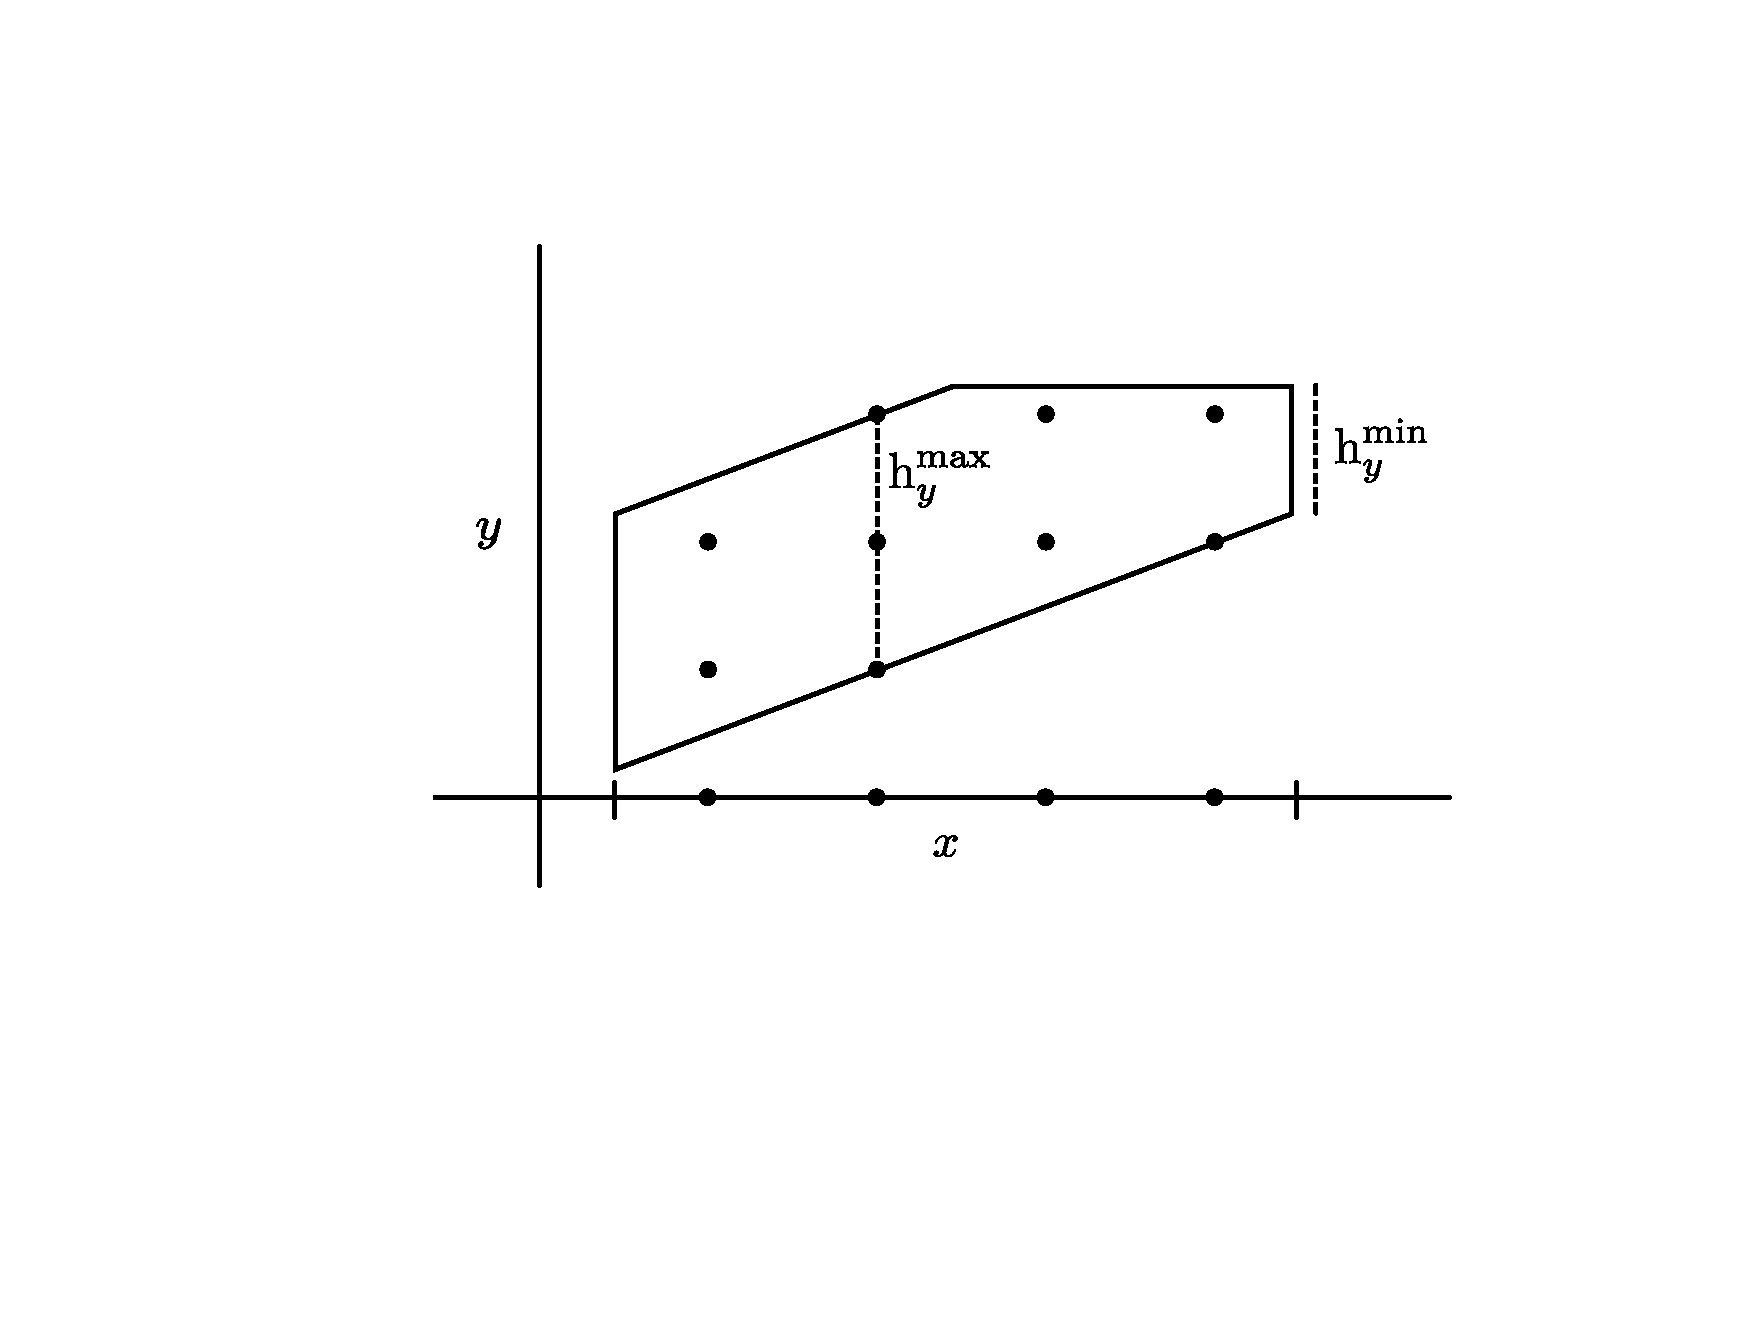
\includegraphics[width=6.5cm]{figures/forget.pdf} % !!! commented out slow figure
\end{center}
\caption{\label{fig:forget} Example of a forget operation in the abstract domain $\ppolys$.  In this case, $\minh{y} = 1$ and $\maxh{y} = 3$.  Note that $\maxh{y}$ is precise while $\minh{y}$ is an under-approximation.  If $\smin{1} = \smax{1} = 9$ then we have $\smin{2} = 3$, $\smax{2} = 4$, $\pmin{2} = \pmin{1} \cdot 1$, $\pmax{2} = \pmax{2} \cdot 4$.}
\end{figure}

Figure \ref{fig:forget} gives an example of a forget operation and
illustrates the quantities $\maxh{y}$ and $\minh{y}$.  If $ \poly_1 =
(\cons_1, V_1) $, the upper bound $\maxh{y}$ can be found by maximizing $y - y'$ subject to the
constraints $\cons_1 \cup \cons_1[y' / y]$, where $y'$ is a fresh variable and $\cons_1[y'/y]$ represents the set of
constraints obtained by substituting $y'$ for $y$ in $\cons_1$.  As our
points are integer-valued, this is an integer linear programming
problem (and can be solved by ILP solvers). A less precise upper bound
can be found by simply taking the extent of the polyhedron $\getpoly{1}$ along $y$,
which is given by $\psize{\pi_y(\getpoly{1})}$.

For the lower bound, it is always sound to use $\minh{y} = 1$. A more
precise estimate can be obtained by treating the convex polyhedron as
a subset of $ \Real^n $ and finding the vertex with minimal height
along dimension $y$. Call this distance $u$. An example of this
quantity is labeled $ \minh{y} $ in \fref{fig:forget}. Since the shape
is convex, all other points will have $y$ height greater than or equal
to $u$. We then find the smallest number of integer points that can be
covered by a line segment of length $u$. This is given by $\lceil u
\rceil - 1$.  The final under-approximation is then taken to be the
larger of $ 1 $ and $ \lceil u \rceil -1 $. As this method requires us
to inspect every vertex of the convex polyhedron and to compute the
$y$ height of the polyhedron at that vertex, we can also look for the
one upon which the polyhedron has the greatest height, providing us
with the estimate for $ \maxh{y} $.

\begin{lemma}
\label{lem:pp:forget}
If $\delta \in \ppconc{\pp{}}$ then $\forget{y}{\delta} \in
\ppconc{\forget{y}{\pp{}}}$.
\end{lemma}
\noindent
We can define an abstract version of projection using forget:
\begin{definition}
Let $\forget{\{x_1,x_2,\ldots,x_n\}}{\pp{}} =
\forget{\{x_2,\ldots,x_n\}}{\forget{x_1}{\pp{}}}$.  Then
$\project{\pp{}}{V'} = \forget{(\fv{\pp{}} - V')}{\pp{}}$. 
\end{definition}
That is, in order to project onto the set of variables $V'$, we forget
all variables not in $V'$.

\subsubsection{Assignment}
The concrete assignment operation is defined so that the probability
of a state $ \sigma $ is the accumulated probability mass of all
states $ \tau $ that lead to $ \sigma $ via the assignment:
$$ \delta \bparen{x \ra \aexp} \defeq \lambda \sigma \lsep \sum_{\tau \given \tau
  \bparen{x \ra \eeval{\aexp}{\tau}} = \sigma} \delta (\tau) $$

The abstract implementation of this operation strongly depends on the
invertibility of the assignment. Intuitively, the set $ \set{\tau
  \given \tau \bparen{x \ra \eeval{\aexp}{\tau}}=\sigma} $ can be
obtained from $ \sigma $ by inverting the assignment, if
invertible.\footnote{An assignment $
  \sassign{x}{E} $ is invertible if there exists an \emph{inverse}
  function $ f:\states \ra \states $ such that $
  f\paren{\evalp{\sassign{x}{E}}{\sigma}} = \sigma $ for all
  $\sigma$. Note that the $ f $ here needs not be expressible as an
  assignment in our (integer-based) language, and generally would not
  be as most integers have no integer multiplicative
  inverses.} Otherwise, the set can be obtained by \emph{forgetting}
about the $ x $ variable in $ \sigma $.

Similarly, we have two cases for abstract assignment. If
$\sassign{x}{E}$ is invertible, the result of the
assignment $\pp{1} \bparen{x \ra E}$ is the probabilistic polyhedron
$\pp{2}$ such that $\getpoly{2} = \getpoly{1} \bparen{x \ra E}$ and
all other components are unchanged.
%
If the assignment is not invertible, then information about the
previous value of $x$ is lost.  In this case, we forget $ x $ thereby
projecting (or ``flattening'') onto the other dimensions. Then we
introduce dimension $ x $ back and add a constraint on $x$ that is
defined by the assignment. More precisely the process is as
follows. Let $\pp{2} = \forget{x}{\pp{1}}$ where $\poly_2 = (\cons_2,
V_2)$.  Then $\pp{1} \bparen{x \ra E}$ is the probabilistic polyhedron
$\pp{3}$ with $ \poly_3 = (\cons_2 \cup \set{x = E}, V_2 \cup
\set{x})$ and all other components as in $\pp{2}$.

The test for invertibility itself is simple as our system restricts
arithmetic expressions to linear ones. Invertibility relative to a
variable $ x $ is then equivalent to the presence of a non-zero
coefficient given to $ x $ in the expression on the right-hand-side
of the assignment. For example, $ \sassign{x}{42 x + 17y} $ is
invertible but $ \sassign{x}{17y} $ is not.

\begin{lemma}
\label{lem:pp:assign}
If $\delta \in \ppconc{\pp{}}$ then $\delta \bparen{v \ra \aexp} \in \ppconc{\pp{} \bparen{v \ra \aexp}}$.
\end{lemma}

The soundness of assignment relies on the fact that our
language of expressions does not include division.  An invariant of
our representation is that $\smax{} \leq \psize{\poly}$.  
% That is,
% there can never be more than $\psize{\poly}$ support points in a
% probabilistic polyhedron with polyhedral portion $\poly$.  
When $E$ contains only multiplication and addition the
above rules preserve this invariant; an $E$ containing division would
violate it. 
Division would collapse multiple points to one and so could be handled
similarly to projection.

\subsubsection{Plus}
The concrete plus operation adds together the mass of two
distributions:
$$ \delta_1 + \delta_2 \defeq \lambda \sigma \lsep \delta_1(\sigma) +
\delta_2(\sigma) $$

The abstract counterpart needs to 
over-approximate this semantics. Specifically, if $\delta_1 \in
\ppconc{\pp{1}}$ and $\delta_2 \in \ppconc{\pp{2}}$ then $\delta_1 +
\delta_2 \in \ppconc{\pp{1} + \pp{2}}$.

% We illustrate abstract plus with the example in Figure
% \ref{fig:pplus}, which shows two overlapping probabilistic
% polyhedra.  
The abstract sum of two probabilistic polyhedra can be easily defined
if their support regions do not overlap. In such situations, we would
define $ \pp{3} $ as below:
\[\begin{array}{lcl}
\getpoly{3} &=& \pa \pjoin \pb \\
\pmin{3} &=& \minparen{\pmin{1}, \pmin{2}} \\
\pmax{3} &=& \maxparen{\pmax{1}, \pmax{2}} \\
\smin{3} &=& \smin{1} + \smin{2} \\
\smax{3} &=& \smax{1} + \smax{2} \\
\mmin{3} &=& \mmin{1} + \mmin{2} \\
\mmax{3} &=& \mmax{1} + \mmax{2}
\end{array}\]

If there is overlap between $ \getpoly{1} $ and $ \getpoly{2} $, the
situation becomes more complex. To soundly compute the effect of plus
we need to determine the minimum and maximum number of points in the
intersection that may be support points for both $\ppa$ and for
$\ppb$.  We refer to these counts as the \emph{pessimistic overlap}
and \emph{optimistic overlap}, respectively, and define them below.

\begin{definition}
\label{def:abs-overlap}
  Given two distributions $\delta_1,\delta_2$, we refer to the set of
  states that are in the support of both $\delta_1$ and $\delta_2$ as
  the \emph{overlap} of $\delta_1,\delta_2$.  The \emph{pessimistic
    overlap} of $\ppa$ and $\ppb$, denoted $\pessoverlap{\ppa}{\ppb}$,
  is the cardinality of the smallest possible overlap for any distributions
  $\delta_1 \in \ppconc{\ppa}$ and $\delta_2 \in \ppconc{\ppb}$.  The
  \emph{optimistic overlap} $\optoverlap{\ppa}{\ppb}$ is the cardinality of the largest possible
  overlap.  Formally, we define these as follows. .% $n_1 \defeq \psize{\pa} - n_3 \bigstrut$, and
%  $n_2 \defeq \psize{\pb} - n_3 \bigstrut[t]$.
%\[\begin{array}{l}
%\pessoverlap{\ppa}{\ppb} \defeq \maxparen{(\smin{1} - n_1) + (\smin{2} - n_2) -
%n_3,\ 0} \\
%\optoverlap{\ppa}{\ppb} \defeq \minparen{\smax{1}, \smax{2}, n_3} \\
%\end{array}\]
\[\begin{array}{l}
\pessoverlap{\ppa}{\ppb} \defeq \maxparen{ \smin{1} +
\smin{2} - \paren{\psize{\pa} + \psize{\pb} - \psize{\pa
    \pmeet \pb} \bigstrut[b] } ,\ 0} \\
\optoverlap{\ppa}{\ppb} \defeq \minparen{\smax{1}, \smax{2}, \psize{\pa
    \pmeet \pb} \bigstrut[b]} \\
\end{array}\]

\end{definition}

The pessimistic overlap is derived from the usual inclusion-exclusion
principle: $ \setsize{A \cap B} = \setsize{A} + \setsize{B} -
\setsize{A \cup B} $.
%, noting that the definition of the pessimistic
%overlap, save for the $ \max $, can be rearranged into $ \smin{1} +
%\smin{2} - \paren{\psize{\pa} + \psize{\pb} - n_3} $. 
The optimistic overlap is trivial; it cannot exceed the support size of either
distribution or the size of the intersection.

We can now define abstract addition.

\begin{definition}
\label{def:pplus}
If not $ \iszero{\pp{1}} $ and not $ \iszero{\pp{2}} $ then $\ppa \ppplus \ppb$ is the probabilistic polyhedron $\pp{3} = (\getpoly{3},\smin{3},\smax{3},\pmin{3},\pmax{3})$ defined as follows.
\[
\begin{array}{lcl}
\getpoly{3} &=& \pa \pjoin \pb \bigstrut \\
\pmin{3} &=& 
\begin{cases}
\pmin{1} + \pmin{2} & \text{if } \pessoverlap{\ppa}{\ppb} = \psize{\getpoly{3}} \bigstrut[t] \\
\minparen{\pmin{1}, \pmin{2}} & \text{otherwise}\bigstrut[b] 
\end{cases} \bigstrut \\

\pmax{3} &=&
\begin{cases}
\pmax{1} + \pmax{2} & \text{if } \optoverlap{\ppa}{\ppb} > 0 \bigstrut[t] \\
\maxparen{\pmax{1}, \pmax{2}} & \text{otherwise}\bigstrut[b]
\end{cases} \bigstrut \\

\smin{3} &=& \maxparen{\smin{1} + \smin{2} - \optoverlap{\ppa}{\ppb},
  \; 0} \bigstrut \\

\smax{3} &=& \minparen{\smax{1} + \smax{2} - \pessoverlap{\ppa}{\ppb},
\; \psize{\getpoly{3}}} \bigstrut \\

\mmin{3} &=& \mmin{1} + \mmin{2} \bigstrut \quad \mid \quad
\mmax{3} = \mmax{1} + \mmax{2} \bigstrut  \\
\end{array}
\]

If $ \iszero{\pp{1}}$ then we define $ \ppa \ppplus \ppb $ as identical 
to $ \ppb $; if $ \iszero{\pp{2}} $, the sum is defined as
identical to $ \pp{1} $. 
\end{definition}

\begin{lemma} \label{lem:pp:plus}
If $\delta_1 \in \ppconc{\pp{1}}$ and $\delta_2 \in \ppconc{\pp{2}}$ then $\delta_1 + \delta_2 \in \ppconc{\pp{1} + \pp{2}}$.
\end{lemma}

\deleted{
\subsubsection{Abstract Union (aka Join)}
 
We next define our abstract join operation, which approximates the set operation $D_1 \cup D_2$.
 
\begin{definition}
The \emph{abstract join} of probabilistic polyhedra $\ppa$ and $\ppb$,
denoted $\ppa \ppcup \ppb$, is the probabilistic polyhedron $\ppc =
(P_3,\pmin{3},\pmax{3},\smin{3},\smax{3})$ defined as follows.
\begin{itemize}
\item{} $ \poly_3 = \pa \pjoin \pb $
\item{} $ \pmin{3} = \minparen{\pmin{1},\pmin{2}}$
\item{} $ \pmax{3} = \maxparen{\pmax{1},\pmax{2}}$
\item{} $ \smin{3} = \minparen{\smin{1},\smin{2}}$
\item{} $ \smax{3} = \maxparen{\smax{1},\smax{2}}$
\end{itemize}
\end{definition}
}

\subsubsection{Product}
The concrete product operation merges two distributions over distinct
variables into a compound distribution over the union of the
variables:
$$ \delta_1 \times \delta_2 \defeq \lambda(\sigma_1, \sigma_2) \lsep
\delta_1(\sigma_1) \cdot \delta_2(\sigma_2) $$

When evaluating the product $\pp{3} = \pp{1} \times \pp{2}$, we assume
that the domains of $\pp{1}$ and $\pp{2}$ are disjoint, i.e.,
$\poly_1$ and $\poly_2$ refer to disjoint sets of 
variables.  If $ \poly_1 = (\cons_1, V_1) $ and $ \poly_2 = (\cons_2,
V_2) $, then the polyhedron $\poly_1 \pprod \poly_2 \defeq
\paren{\cons_1 \cup \cons_2, V_1 \cup V_2}$ is the Cartesian product
of $\poly_1$ and $\poly_2$ and contains all those states $\sigma$ for
which $\project{\sigma}{V_1} \in \pconc{\poly_1}$ and
$\project{\sigma}{V_2} \in \pconc{\poly_2}$. 
Determining the remaining components is straightforward since $\pp{1}$
and $\pp{2}$ are disjoint. 
\[
\begin{array}{rcl@{\hspace{0.35cm}}|@{\hspace{0.35cm}}rcl}
\multicolumn{6}{c}{\poly_3\ =\ \poly_1 \pprod \poly_2} \bigstrut[b] \\
\pmin{3} &=& \pmin{1} \cdot \pmin{2} &
\pmax{3} &=& \pmax{1} \cdot \pmax{2} \bigstrut \\
\smin{3} &=& \smin{1} \cdot \smin{2} &
\smax{3} &=& \smax{1} \cdot \smax{2} \bigstrut \\
\mmin{3} &=& \mmin{1} \cdot \mmin{2} &
\mmax{3} &=& \mmax{1} \cdot \mmax{2} \bigstrut[t]
\end{array}
\]

\begin{lemma}
\label{lem:pp:product}
For all $\pp{1}, \pp{2}$ such that $\fv{\pp{1}} \cap
\fv{\pp{2}} = \emptyset$, if $\delta_1 \in \ppconc{\pp{1}}$ and
$\delta_2 \in \ppconc{\pp{2}}$ then $\delta_1 \times \delta_2
\in \ppconc{\pp{1} \times \pp{2}}$. 
\end{lemma}

In our examples we often find it useful to express uniformly distributed
data directly, rather than encoding it using $\spifk$.  In particular,
we extend statements $S$ to include the statement of the form
$\suniform{x}{n_1}{n_2}$ whose semantics is to define variable $x$ as
having a value uniformly distributed between $n_1$ and $n_2$.
$$
\begin{array}{rcl}
\abspevalp{\suniform{x}{n_1}{n_2}}{\pp{1}} & = & \forget{x}{\pp{1}}
\times \pp{2}
\end{array}
$$
Here, $ \pp{2} $ has $ \pmin{2} = \pmax{2} = \frac{1}{n_2 - n_1 + 1}
$, $ \smin{2} = \smax{2} = n_2 - n_1 + 1 $, $ \mmin{2} = \mmax{2} = 1
$, and $ C_2 = (\set{x \geq n_1, x \leq n_2}, \set{x}) $.

We will say that the abstract semantics correspond to the concrete
semantics of $ \suniformname $ defined similarly as follows.
$$
\begin{array}{rcl}
\pevalp{\suniform{x}{n_1}{n_2}}{\delta} & = &
\paren{\project{\delta}{\fv{\delta} - \set{x}}} \times \delta_2
\end{array}
$$
where $ \delta_2 = (\lambda \sigma. \aif n_1 \leq \sigma(x)
\leq n_2 \athen \frac{1}{n_2 - n_1 + 1} \aelse 0)$.

The soundness of the abstract semantics follows immediately from the
soundness of forget and product.

\subsubsection{Conditioning}

\newcommand{\nn}{\overline{n}} 
\newcommand{\nnu}{\underline{n}} 

The concrete conditioning operation restricts a distribution to a
region defined by a boolean expression, nullifying any probability mass outside it:
$$ \dcond{\delta}{\bexp} \defeq \lambda \sigma \lsep \aif \eeval{\bexp}{\sigma} \athen
\delta(\sigma) \aelse 0 $$

Distribution conditioning for probabilistic polyhedra serves the same
role as meet in the classic domain of polyhedra in that each is used
to perform abstract evaluation of a conditional expression in its
respective domain.

\begin{definition}
  Consider the probabilistic polyhedron $\ppa$ and Boolean expression
  $\bexp$.  Let $n,\nn$ be such that $n = \absecount{\bexp}{\getpoly{1}}$ and
  $\nn = \absecount{(\neg\bexp)}{\getpoly{1}}$.  
The value $n$ is an over-approximation of the number of points in
$\getpoly{1}$ that satisfy the condition $\bexp$ and $\nn$ is an
over-approximation of the number of points in $\getpoly{1}$ that do
not satisfy $\bexp$.
Then $\absdcond{\ppa}{\bexp}$ is the probabilistic polyhedron $\ppb$
  defined as follows.
\[
\setlength{\arraycolsep}{1pt}
\begin{array}{lcl@{\hspace{0.35cm}}|@{\hspace{0.35cm}}lcl}
\pmin{2} &=& \pmin{1} &
\smin{2}\ &=&\ \maxparen{\smin{1} - \nn, 0}\\
\pmax{2} &=& \pmax{1} \bigstrut[b] &
\smax{2} &=&\ \minparen{\smax{1}, n} \bigstrut \\
%\mmin{2} &=& \multicolumn{4}{l}{\max\tparen{\pmin{2} \cdot
%\smin{2},\ \mmin{1} - \pmax{1} \cdot \nn}} \bigstrut\\
\mmin{2} &=& \multicolumn{4}{l}{\maxparen{\pmin{2} \cdot
    \smin{2},\ \mmin{1} - \pmax{1} \cdot \minparen{\smax{1}, \nn}}} \bigstrut\\
%\mmax{2} &=& \multicolumn{4}{l}{\min\tparen{\pmax{2} \cdot
%\smax{2},\ \mmax{1} - \pmin{1} \cdot \nnu}} \bigstrut\\
\mmax{2} &=& \multicolumn{4}{l}{\minparen{\pmax{2} \cdot
    \smax{2},\ \mmax{1} - \pmin{1} \cdot \maxparen{\smin{1}-n, 0}}} \bigstrut\\
\getpoly{2} &=& \multicolumn{4}{l}{\abseeval{\bexp}{\pa}} \bigstrut[t] \\
\end{array}
\]
\end{definition}

The maximal and minimal probability per point
are unchanged, as conditioning simply retains points from
the original distribution.  To compute the minimal number of points in
$\pp{2}$, we assume that
as many points as possible from $\getpoly{1}$ fall in the region
satisfying $\neg\bexp$.  The maximal number of points is obtained by
assuming that a maximal number of points fall within the region
satisfying $\bexp$.

The total mass calculations are more complicated.  There are two
possible approaches to computing $\mmin{2}$ and $\mmax{2}$.  The bound
$\mmin{2}$ can never be less than $\pmin{2} \cdot \smin{2}$, and so we
can always safely choose this as the value of $\mmin{2}$.  Similarly,
we can always choose $\pmax{2} \cdot \smax{2}$ as the value of
$\mmax{2}$.  However, if $\mmin{1}$ and $\mmax{1}$ give good bounds on
total mass (i.e., $\mmin{1}$ is much higher than $\pmin{1} \cdot
\smin{1}$ and dually for $\mmax{1}$), then it can be advantageous to
reason starting from these bounds.

We can obtain a sound value for $\mmin{2}$ by considering the case
where a maximal amount of mass from $\getpoly{1}$ fails to satisfy
$B$.  To do this, we compute $\nn =
\absecount{\neg\bexp}{\getpoly{1}}$, which provides an
over-approximation of the number of points within $\getpoly{1}$ but
outside the area satisfying $B$.  We bound $\nn$ by $\smax{1}$ and
then assign each of these points maximal mass $\pmax{1}$, and subtract
this from $\mmin{1}$, the previous lower bound on total mass.

By similar reasoning, we can compute $\mmax{2}$ by assuming a minimal
amount of mass $m$ is removed by conditioning, and subtracting $m$
from $\mmax{1}$.  This $m$ is given by considering an
under-approximation of the number of points falling outside the area
of overlap between $\getpoly{1}$ and $B$ and assigning each point
minimal mass as given by $\pmin{1}$.  This $m$ is given by
$\max\tparen{\smin{1}-n, 0}$.

\begin{figure}
\begin{center}
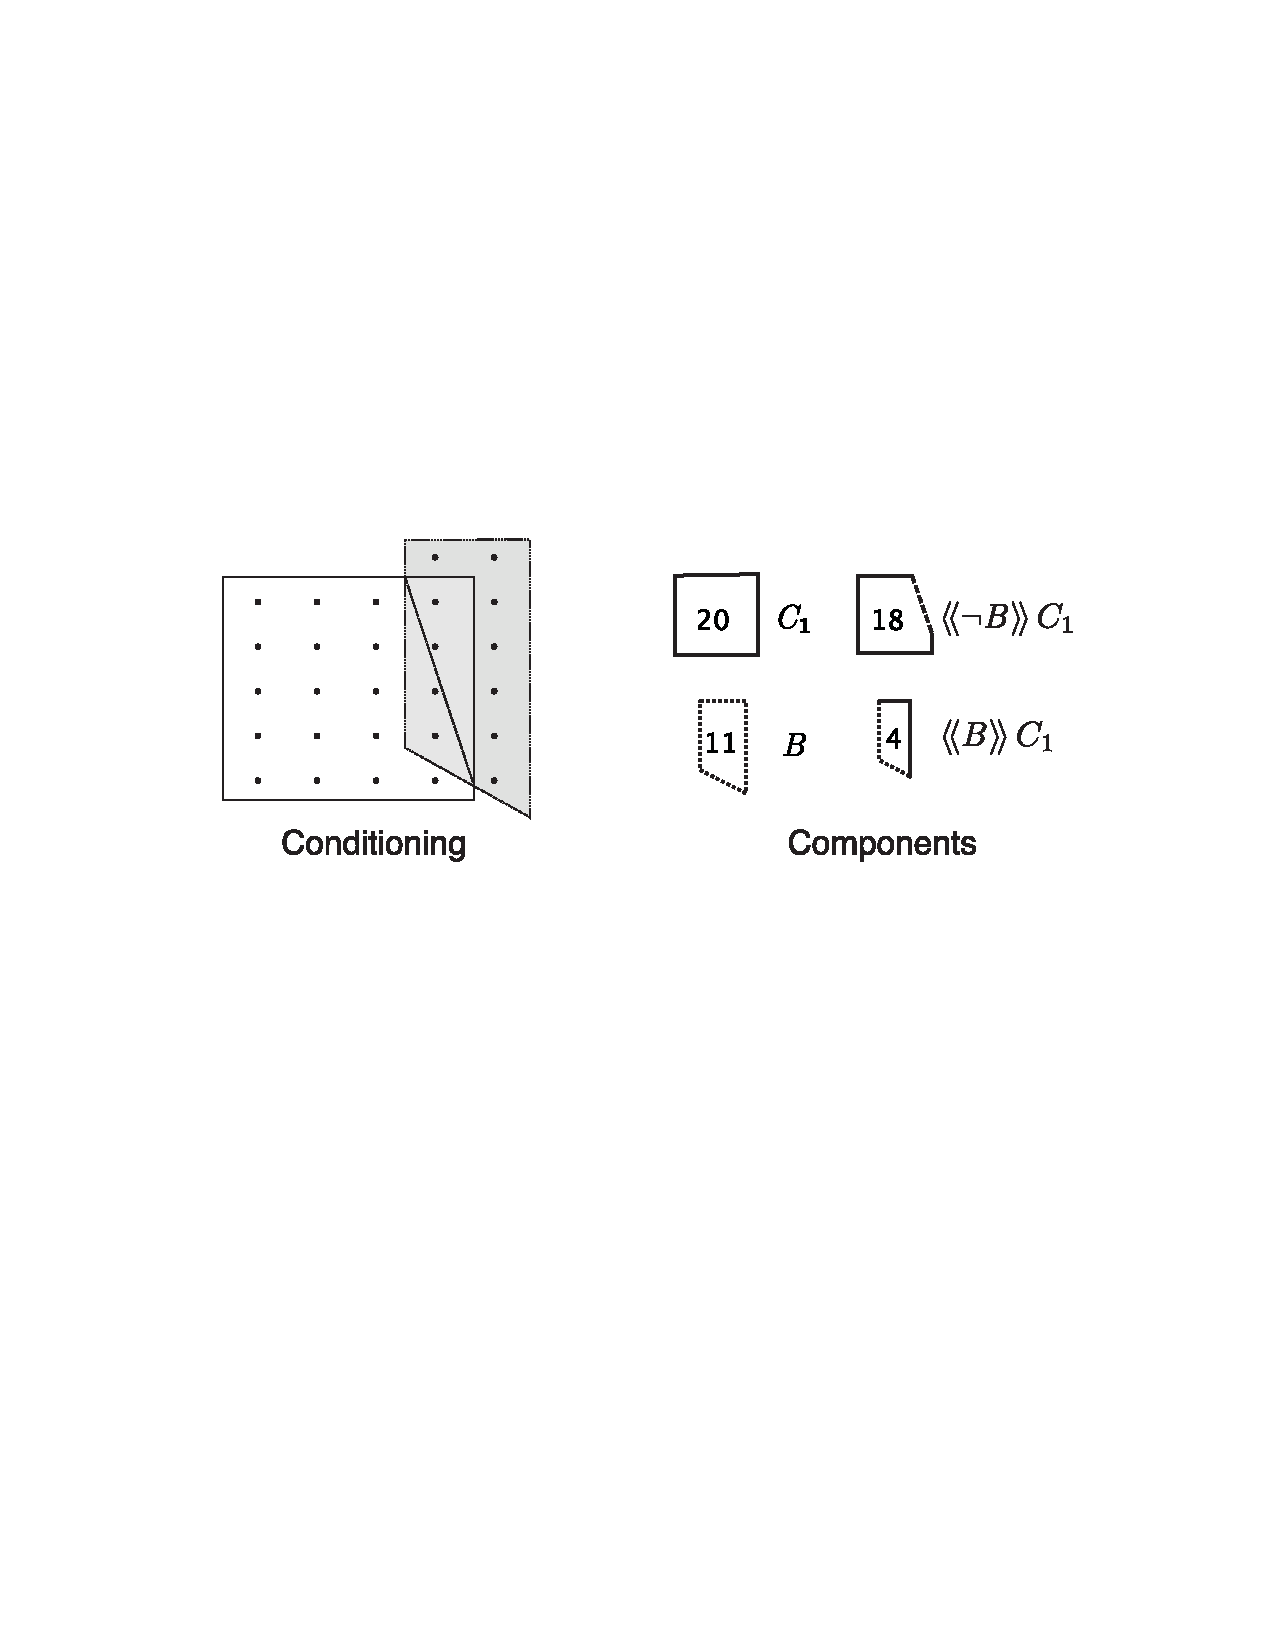
\includegraphics[width=7.5cm]{figures/conditioning-smaller.pdf}
\end{center}
\caption{\label{fig:conditioning} Example of distribution conditioning in the abstract domain $\ppolys$.}
\end{figure}

Figure \ref{fig:conditioning} demonstrates the components that affect the
conditioning operation.  The figure depicts the integer-valued points
present in two polyhedra---one representing $\getpoly{1}$ and the other
representing $\bexp$ (shaded).  As the set of points in $\getpoly{1}$
satisfying $\bexp$ is convex, 
this region is precisely represented by $\abseeval{\bexp}{\getpoly{1}}$.  By contrast, the set of points
in $\getpoly{1}$ that satisfy $\neg\bexp$ is not convex, and thus $\abseeval{\neg\bexp}{\getpoly{1}}$ is an
over-approximation.  The icons
beside the main image indicate which shapes correspond to which components
and the numbers within the icons give the total count of points within those
shapes.

Suppose the components of $\pp{1}$ are as follows.
\[
\begin{array}{l@{\qquad}l@{\qquad}l}
\smin{1} = 19 & \pmin{1} = 0.01 & \mmin{1} = 0.85 \\
\smax{1} = 20 & \pmax{1} = 0.05 & \mmax{1} = 0.9
\end{array}
\]
Then $n = 4$ and $\nn = 16$.  Note that we have set $\nn$ to be the
number of points in the non-shaded region of Figure \ref{fig:conditioning}.
This is more precise than the count given by $\psize{\abseeval{\bexp}{\poly}}$, which
would yield $18$.  This demonstrates why it is worthwhile to have a
separate operation for counting points satisfying a boolean expression.
These values of $n$ and $\nn$ give us the following for
the first four numeric components of $\pp{2}$.
\[
\begin{array}{l@{\qquad}l}
\smin{2} = \max(19 - 16, 0) = 3 & \pmin{2} = 0.01 \\
\smax{2} = \min(20,4) = 4 & \pmax{2} = 0.05
\end{array}
\]
For the $\mmin{2}$ and $\mmax{2}$, we have the following for the
method of calculation based on $\mathrm{p^{min/max}_2}$ and
$\mathrm{s^{min/max}_2}$.
\[
\begin{array}{l@{\qquad}l}
\mmin{2} = 0.01 \cdot 3 = 0.03  & \mmax{2} = 0.05 \cdot 4 = 0.2
\end{array}
\]
For the method of computation based on $\mathrm{m^{min/max}_1}$, we have
\[
\begin{array}{llcrr}
\mmin{2} &= &0.85 - 0.05 \cdot 16& =& 0.05\\
 \mmax{2} &= &0.9 - 0.01 \cdot (19-4)& =& 0.75
\end{array}
\]

In this case, the calculation based on subtracting from total mass
provides a tighter estimate for $\mmin{2}$, while the method based on
multiplying $\pmax{2}$ and $\smax{2}$ is better for
$\mmax{2}$.

\begin{lemma} \label{lem:pp:cond} If $ \delta \in \ppconc{\pp{}} $ then $
  \dcond{\delta}{B} \in \ppconc{\absdcond{\pp{}}{B}} $.
\end{lemma}


% \paragraph{Benefits of dual mass representations}

% The total minimum mass of a probabilistic polyhedron can seemingly be
% determined using two redundant means: either $ \mmin{} $ or $ \pmin{}\cdot \smin{} $. Tracking the measure in these two ways, however, is useful for
% keeping the measure accurate. For some abstract operations one of
% these means is more accurate than the other.

% Any abstract plus operation involving probabilistic polyhedra having
% two different minimum probability per point measures, the total mass
% based approach is more accurate, or equivalently accurate in the rare
% case where the minimum number of points is identical to the number of
% points in the polyhedra.

% \sbmcomment{It might be easier to read if we convert the fractions to decimals.}

% \begin{example} Consider two disjoint probabilistic polyhedra $ \ppa $, $ \ppb $,
% with the following characteristics:

% $ \pmin{1} = \frac{1}{100} $

% $ \smin{1} = 10 $

% $ \mmin{1} = \frac{10}{100} $

% $ \pmin{2} = \frac{1}{200} $

% $ \smin{2} = 20 $

% $ \mmin{2} = \frac{20}{100} $

% $ \pa \cap \pb = \emptyset $

% The abstract plus of the two, $ \ppc := \ppa \ppplus \ppb $ has the
% following properties.

% $ \pmin{3} = \frac{1}{200} $

% $ \smin{3} = 30  $

% $ \mmin{3} = \frac{30}{100} $

% Note that $ \pmin{3} \cdot \smin{3} = \frac{15}{100} $, a more inaccurate
% measure than $ \mmin{3} = \frac{30}{100} $.
% \end{example}

% The difference in the two total mass approaches stems from the need to
% under-approximate both minimum probability per point from both
% polyhedra with a single value.

% For abstract plus, the total mass approach always produces more
% accurate results but in the case of abstract revision, the approach
% can, in some cases, produce results worse than the $ \pmin{}\cdot \smin{} $ approach. First let us look at an example in which the total mass is
% still more accurate.

% \begin{example} Consider a probabilistic polyhedron $ \ppa $ and a
% polyhedron $ \pb $ where the intersection between the two is quite
% large in relation to the size of $ \pa $. 

% $ \pmin{1} = \frac{1}{1000} $

% $ \pmax{1} = \frac{1}{100} $

% $ \smin{1} = 95 $

% $ \mmin{1} = \frac{20}{100} $

% Furthermore, $ \setsize{\pa} - \setsize{\pa \cap \pb} = 10 $ and
% $ \setsize{\pa \cap \pb} = 90 $. That is, the $ \pa $ contains 100
% points, 90 of which are in the intersection with $ \pb $.

% To determine the total mass of $ \ppc := \absdcond{\ppa}{\pb} $ we
% reason that a maximum amount of mass falls outside the intersection,
% corresponding to $ \pmax{1} \cdot \paren{\setsize{\pa}
% - \setsize{\pa \cap \pb}} = \frac{1}{100} \cdot 10 $ .  \sbmcomment{I think you mean \textit{minimal} total mass here.}
% Thus the total
% mass of the intersection would be $ \mmin{1} - \frac{10}{100}
% = \frac{10}{100} $. On the other hand, $ \pmin{3} \cdot \smin{3}
% = \frac{1}{1000} \cdot 85 < \frac{10}{100} $.
% \end{example}

% As seen in the example above, the calculation of total mass derives
% it's accuracy from the maximum estimates as applied to the area
% outside of the intersection. If, however, this area is instead large,
% we see that this approach fails.

% \begin{example}

% Consider a probabilistic polyhedron $ \ppa $ and a
% polyhedron $ \pb $ where the intersection between the two is small in relation to the size of $ \pa $. 

% $ \pmin{1} = \frac{1}{1000} $

% $ \pmax{1} = \frac{1}{100} $

% $ \smin{1} = 95 $

% $ \mmin{1} = \frac{20}{100} $

% Furthermore, $ \setsize{\pa} - \setsize{\pa \cap \pb} = 90 $ and
% $ \setsize{\pa \cap \pb} = 10 $. That is, the $ \pa $ contains 100
% points, 10 of which are in the intersection with $ \pb $.

% To determine the total mass of $ \ppc := \absdcond{\ppa}{\pb} $ we
% reason that a maximum amount of mass falls outside the intersection,
% corresponding to $ \pmax{1} \cdot \paren{\setsize{\pa}
% - \setsize{\pa \cap \pb}} = \frac{1}{100} \cdot 90 $ . Thus the total
% mass of the intersection would be $ \mmin{1} - \frac{90}{100}
% = - \frac{70}{200} $, or simply a value having no use whatsoever. On the other hand, $ \pmin{3} \cdot \smin{3}
% = \frac{85}{1000} $. In such a case, we let $ \mmin{3}
% := \pmin{3} \cdot \smin{3} $ in order for the total mass measure to have
% potential usefulness in further computation.
% \end{example} 

\subsubsection{Scalar Product}
The scalar product is straightforward both in the concrete and
abstract sense; it just scales the mass per point and total mass:
$$ p \cdot \delta \defeq \lambda \sigma \lsep p \cdot \delta(\sigma) $$

\begin{definition}
Given a scalar $p$ in $(0,1]$, we write $p \cdot \ppa$ for the probabilistic polyhedron $\ppb$ specified below.
\[
\begin{array}{lcl@{\hspace{0.5cm}}|@{\hspace{0.5cm}}lcl}
\smin{2} &=& \smin{1} & \pmin{2} &=& p \cdot \pmin{1} \\
\smax{2} &=& \smax{1} & \pmax{2} &=& p \cdot \pmax{1} \\
\mmin{2} &=& p \cdot \mmin{1} & \getpoly{2} &=& \getpoly{1}\\
\mmax{2} &=& p \cdot \mmax{1} 
\end{array}
\]

If $ p = 0 $ then $ p \cdot \ppb $ is defined instead as below:
\[
\begin{array}{lcl@{\hspace{0.5cm}}|@{\hspace{0.5cm}}lcl}
\smin{2} &=& 0 & \pmin{2} &=& 0 \\
\smax{2} &=& 0 & \pmax{2} &=& 0 \\
\mmin{2} &=& 0 & \getpoly{2} &=& \pzero \\
\mmax{2} &=& 0 
\end{array}
\]
\end{definition}
Here $ \pzero $ refers to a convex polyhedra (over the same dimensions
as $ \getpoly{2} $) whose concretization is empty.

\begin{lemma}
\label{lem:pp:scalar-prod}
If $\delta_1 \in \ppconc{\pp{1}}$ then $p \cdot \delta_1 \in \ppconc{p \cdot \pp{1}}$.
\end{lemma}

\subsubsection{Normalization}
The normalization of a distribution produces a true probability
distribution, whose total mass is equal to $ 1 $:
$$ \normal{\delta} \defeq \frac{1}{\pmass{\delta}} \cdot \delta $$

If a probabilistic polyhedron $\pp{}$ has $\mmin{} = 1$ and $\mmax{} =
1$ then it represents a normalized distribution.  We define below an
abstract counterpart to distribution normalization, capable of
transforming an arbitrary probabilistic polyhedron into one containing
only normalized distributions.
% , with the property that if $\delta \in
% \ppconc{\pp{}}$ then $\normal{\delta} \in \ppconc{\normal{\pp{}}}$.
% This ensures that $\normal{\pp{}}$ is a sound over-approximation of
% $\normal{\delta}$ for the purposes of policy evaluation.

\begin{definition}
Whenever $ \mmin{1} > 0 $, we write $\normal{\pp{1}}$ for the
probabilistic polyhedron $\pp{2}$ specified below.
\[
\begin{array}{lcl@{\hspace{0.35cm}}|@{\hspace{0.35cm}}lcl}
\pmin{2} &=& \pmin{1} / \mmax{1} &
\smin{2} &=& \smin{1}\\
\pmax{2} &=& \pmax{1} / \mmin{1} &
\smax{2} &=&\smax{1} \\
\mmin{2} &=& \mmax{2} = 1 & \getpoly{2} &=& \getpoly{1} \\
\end{array}
\]
\end{definition}

When $ \mmin{1} = 0 $, we set $\pmax{2} = 1$.  Note that if $\pp{1}$
is the zero distribution then $\normal{\pp{1}}$ is not defined.

The normalization operator illustrates the key novelty of our
definition of probabilistic polyhedron: to ensure that the
overapproximation of a state's probability ($\pmax{}$) is sound, we
must divide by the \emph{underapproximation} of the total probability
mass ($\mmin{}$).

\begin{lemma}
\label{lem:pp:norm}
If $\delta_1 \in \ppconc{\pp{1}}$ and $\normal{\delta_1}$ is defined, then $\normal{\delta_1} \in \ppconc{\normal{\pp{1}}}$.
\end{lemma}

\subsection{Policy Evaluation}

\noindent Here we show how to implement the threshold test given as
Definition \ref{def:threshold} using probabilistic polyhedra. To make
the definition simpler, let us first introduce a bit of notation.

\begin{notation} If $ \pp{} $ is a probabilistic polyhedron over
  variables $ V $, and $ \sigma $ is a state over variables $ V'
  \subseteq V $, then $ \absdcond{\pp{}}{\sigma} \defeq
  \absdcond{\pp{}}{\bexp} $ where $ \bexp = \bigwedge_{x \in V'} x =
  \sigma(x) $.
\end{notation}

Recall that we define $\drevise{\delta}{\bexp}$ in the concrete
semantics to be $\normal{\dcond{\delta}{\bexp}}$.  The
corresponding operation in the abstract semantics is similar:
$\absdrevise{\pp{}}{\bexp} \defeq \normal{\absdcond{\pp{}}{\bexp}}$.

\begin{definition} \label{def:poly-threshold}
Given some probabilistic polyhedron $\pp{1}$ and statement $S$, with
low security variables $ L $ and high security variables $ H $, where
$\abspevalp{S}{\pp{1}} $ terminates, let $\pp{2} =
\abspevalp{S}{\pp{1}}$ and $\pp{3} = \project{\pp{2}}{L}$. If, for
every $ \sigma_L \in \pconc{\getpoly{3}} $ with $
\neg\iszero{\absdcond{\pp{2}}{\sigma_L}}$, we have $ \pp{4} =
\project{\paren{\absdrevise{\pp{2}}{\sigma_L}}}{H} $ with $\pmax{4}
\leq t$, then we write $\abspolicy{S}{\pp{1}}{t}$.
\end{definition}

The computation of $\pp{3}$ involves only abstract interpretation and
projection, which are computable using the operations defined previously
in this section.  If we have a small number of outputs (as for the binary outputs
considered in our examples), we can enumerate them and check
$\neg\iszero{\absdcond{\pp{2}}{\sigma_L}}$ for each output $\sigma_L$.
When this holds (that is, the output is feasible), we compute $\pp{4}$,
which again simply involves the abstract operations defined previously.
The final threshold check is then performed by comparing $\pmax{4}$ to
the probability threshold $t$.

Now we state the main soundness theorem for abstract interpretation
using probabilistic polyhedra.  This theorem states that the abstract
interpretation just described can be used to soundly determine whether
to accept a query.

\begin{theorem} \label{thm:pp:secure}
  Let $\delta$ be an attacker's initial belief.  If $\delta \in
  \ppconc{\pp{1}}$ and $\abspolicy{S}{\pp{1}}{t}$, then $S$ is threshold secure
  for threshold $t$ when evaluated with initial belief $\delta$.
\end{theorem}

The proof of this theorem follows from the soundness of the
abstraction (\tref{thm:pp:soundness}), noting the direct parallels of
threshold security definitions for distributions (Definitions
\ref{def:threshold}) and probabilistic polyhedra (Definition
\ref{def:poly-threshold}).

\subsection{Supporting Other Domains, Including Intervals and Octagons} \label{sec:simpler}

Our approach to constructing probabilistic polyhedra from normal
polyhedra can be adapted to add probabilities any other abstract
domain for which the operations defined in \sref{sec:polyhedra} can be
implemented.  Most of the operations listed there are standard to
abstract domains in general, except for the size operation and the
related expression count. Adopting an abstract domain to our system
would therefore only require designing these counting methods for the
new domain.

Two domains that are very easy to adapt that are in common use are
intervals and octagons.  \emph{Intervals} \cite{cousot76static},
$\intdomain$, are convex shapes that can be described as a set of
closed intervals, one for each dimension. Alternatively they can be
thought of a restricted form of polyhedra in which the constraints $I$
all have the form $ a \leq x \leq b $. Operations on intervals are
much faster than on polyhedra. Specific to our requirements, counting
the integer points inside interval regions and determining their
height for the forget operation are both trivial computations.

\emph{Octagons} \cite{mine01octagon}, $\octadomain$, are formed by
constraints $O$ that have the form $ a x + b y \leq c $ where $ a,b
\in \set{-1,0,1} $.  In two dimensions these shapes, appropriately,
have at most 8 sides. If the number of dimensions is fixed, the number
of constraints and the number of vertices of an octagon are
bounded. Furthermore, the operations on octagons have lower
computational complexity than those for polyhedra, though they are not
as efficient as those for intervals.

\begin{figure}
\begin{center}
\includegraphics[width=6.5cm]{figures/approx_domains.pdf} 
\end{center}
\caption{\label{fig:approx_domains} The (over)approximation of a polyhedron
  using an octagon (left) and an interval (right).}
\end{figure}

Any interval or octagon is also a polyhedron. Conversely, one can
over-approximate any polyhedron by an interval or octagon. Naturally
the smallest over-approximation is of greatest interest.
Examples are illustrated in \fref{fig:approx_domains}.  This fact is
relevant when computing the various equivalent operations to
those listed for polyhedra in Section~\ref{sec:polyhedra}: applying
the definitions given there on octagons/intervals may not necessarily
result in octagons/intervals, and so the result must be further
approximated.  For example, consider the evaluation operation $
\abseeval{\bexp}{I} $.  This must compute a region that contains \emph{at least}
the points in $ I $ satisfying $ \bexp $.  Thus, if a non-octagon/interval
is produced, it can simply be over-approximated.  Another example is
the affine
transform operation $ I \bparen{x \ra \aexp} $, which should
contain \emph{at least} the points $ \tau
= \sigma \bparen{x \ra \aexp} $ with $ \sigma \in \iconc{I} $, where
$ \sigma \bparen{x \ra \aexp} $ is a single state transformed by the
expression $ \aexp $. In general the operations for simpler domains
are much faster than those for more complex domains. Though the imprecision
and thus the need to approximate expression evaluation might
make it occasionally slower, for our experiments any slowdown is
typically overshadowed by the reduced complexity overall.

Thus we can construct abstractions of probability distributions based
on these simpler domains instead of polyhedra. The domain of
probabilistic intervals $ \pintdomain $ (octagons $ \poctadomain $)
is defined as in Section~\ref{def:ppoly}, except using an interval
(octagon) instead of polyhedron for the region constraint.  The
abstract semantics described in this section can then be soundly
implemented in terms of these simpler shapes in place of
polyhedra.

%We write $\ppolys$ for the set of probabilistic polyhedra.  The
%quantities $\smin{}$ and $ \smax{}$ are lower and upper bounds on 
%the number of support points in the polyhedron $\getpoly{}$.  The quantities
%$\pmin{} $ and $ \pmax{} $ are lower and upper bounds on the
%probability mass \emph{per support point}.  The $ \mmin{} $ and $
%\mmax{} $ components give bounds on the total probability mass.  
%Thus $\pp{}$ represents the \emph{set} of distributions
%$\ppconc{\pp{}}$ defined below. 

\begin{remark} If $ \delta \in \ppconc{\pp{}} $ then
$ \delta \in \piconc{\pint} $ and $ \delta \in \poconc{\pocta}
$, where $ \pint $ and $ \pocta $ are identical to $ \pp{} $
except $ \pp{} $ has region constrained by $ C $, a convex
polyhedron, while $ \pint $ is constrained by interval $ C_I $ and
$ \pocta $ is constrained by octagon $ C_O $, with
$ \pconc{C} \subseteq \iconc{C_I} $ and
$ \pconc{C} \subseteq \oconc{C_O} $.
\end{remark}

\section{Powerset of Probabilistic Polyhedra}
\label{sec:probset}

This section presents the $ \ppowers $ domain, an extension of the $ \ppolys
$ domain 
that abstractly represents a set of distributions as at most $ n $
probabilistic polyhedra, elements of $ \ppolys $.

\begin{definition} A \emph{probabilistic (polyhedral) set} $
  \pps{} $ is a set of probabilistic polyhedra, or  $ \set{\pp{i}} $
  with each $ \pp{i} $ over the same variables.\footnote{We write
    $\set{X_i}$ as shorthand for a set of $n$ elements of type $X$, for some
    $n$.  We write $\set{X_i}_{i=1}^{n}$ when the choice of
    $n$ is important.} We write $
  \ppowers $ for the domain of probabilistic polyhedral powersets
  composed of no more than $ n $ probabilistic polyhedra.

Each probabilistic polyhedron $\pp{}$ is interpreted disjunctively: it
characterizes one of many possible distributions.  The probabilistic
polyhedral set is interpreted additively.  To define this idea
precisely, we first define a lifting of $+$ to sets of distributions.  Let $\distset{1}, \distset{2}$ be two sets of distributions.  We then define addition as follows.
\[\distset{1} + \distset{2} = \{\delta_1 + \delta_2 \given \delta_1 \in \distset{1} \wedge \delta_2 \in \distset{2}\}\]
This operation is commutative and associative and thus we can use
$\sum$ for summations without ambiguity as to the order of operations.
The concretization function for $\ppowers$ is then defined as:
$$ \ppsconc{\pps{}} \defeq \sum_{\pp{} \in \pps{}} \ppconc{\pp{}} $$
\end{definition}

Following Monniaux's formulation of a finite sums
abstraction~\cite{Monniaux_these}, elements of $ \pps{} $ need not be
disjoint. While enforcing disjointness would simplify determining the 
most probable points for policy evaluation (see
\sref{sec:poly-eval}), it would necessitate splitting of probabilistic
polyhedra when overlaps arise.  Repeated splitting of already
approximate probabilistic polyhedra decreases their
precision and can hurt performance by increasing the number of regions
to track during abstract interpretation.

We can characterize the condition of $ \pps{} $ containing only the
zero distribution, written $ \iszero{\pps{}} $, via the condition that
all of the member probabilistic polyhedra are zero.
$$ \iszero{\pps{}} \defeq \bigwedge_{\pp{} \in \pps{}} \iszero{\pp{}} $$

\deleted{
\begin{definition} $ \delta_a = \delta_b $ if and only if $ \forall \sigma $ $
  \delta_a(\sigma) = \delta_b(\sigma) $.
\end{definition}
}

\subsection{Abstract Semantics for $\ppowers$} \label{sec:powerset}
The semantics for the powerset abstraction we describe in this section
is designed to soundly approximate the concrete semantics. 

\begin{theorem} \label{thm:ppp:soundness}
For all $\delta, S, \pps{}$, if $\delta \in \ppsconc{\pps{}}$ and $
\abspevalp{S}{\pps{}} $ terminates, then $ \pevalp{S}{\delta} $ terminates and
$\pevalp{S}{\delta} \in
\ppsconc{\abspevalp{S}{\pps{}}}$.
\end{theorem}

The proof for this theorem follows the same form as the corresponding
soundness theorem for probabilistic polyhedra
(\tref{thm:pp:soundness}), via soundness of the individual abstract
operations in relation to their concrete versions. The full proof of
this is given in the companion technical
report~\cite{TR}.

To bound the size of the set of probabilistic polyhedra that
will arise from the various operations that will follow, we introduce a
simplification operation.

\begin{definition}
\label{def:ppp-simp}
The \emph{powerset simplification} transforms a
  set containing potentially more than $ n $ elements into one
  containing no more than $ n $, for $n \geq 1$. The simplest approach involves repeated use
  of abstract plus in the base domain $ \ppolys $.
$$
\simplify{\set{\pp{i}}_{i=1}^{m}}{n} \defeq \left\{
\begin{array}{cc}
\set{\pp{i}}_{i=1}^{m} & \text{if } m \leq n \\
\simplify{\set{\pp{i}}_{i=1}^{m-2} \cup \set{\pp{m-1} + \pp{m}}}{n} & \text{otherwise} \\
\end{array}
\right.
$$
\end{definition}

\begin{lemma}
\label{lem:ppp:bound}
$ \ppsconc{\pps{}} \subseteq \ppsconc{
    \simplify{\pps{}}{m}} $ where $m \leq n$.
\end{lemma}

Note that the order in which individual probabilistic polyhedra are
simplified has no effect on soundness but may impact the precision of
the resulting abstraction. We explore the variation in precision due
to these choices in \sref{sec:perf-analysis}.

Many of the operations and lemmas for the powerset domain are simple liftings
of the corresponding operations and lemmas for single probabilistic polyhedra.
For these operations (the first four, below) we simply list the
definition; we elaborate on the remaining four.

\paragraph{Forget} $ \forget{y}{\pps{}} \defeq
\set{\forget{y}{\pp{}} \given \pp{} \in \pps{}} $

\vspace*{.1in}
\noindent
\myparagraph{Project} $ \project{\pps{}}{V} \defeq
\set{\project{\pp{}}{V} \given \pp{} \in \pps{}} $

% \begin{lemma} 
% If $ \delta \in \ppsconc{\pps{}} $ then $
%   \project{\delta}{\paren{\fv{\delta} - \set{y}}} \in
%   \ppsconc{\forget{y}{\pps{}}} $
% \end{lemma}

\vspace*{.1in}
\noindent
\myparagraph{Assignment} $ \pps{} \bparen{x \ra E} \defeq
  \set{\pp{} \bparen{x \ra E} \given \pp{} \in \pps{}} $

% \begin{lemma} If $ \delta \in \ppsconc{\pps{}} $ then $
%   \delta\bparen{x \ra E} \in \ppsconc{\pps{} \bparen{x \ra E}} $.
% \end{lemma}

\vspace*{.1in}
\noindent
\myparagraph{Scalar product} $ p \cdot \pps{} \defeq \set{p
  \cdot \pp{} \given \pp{} \in \pps{} \wedge \neg \iszero{p \cdot \pp{}}} $

% \begin{lemma} If $ \delta \in \ppsconc{\pps{}} $ then $
%   p \cdot \delta \in \ppsconc{p \cdot \pps{}} $.
% \end{lemma}

\paragraph{Conditioning}
Recall that for probabilistic polyhedra, conditioning $
\absdcond{\pp{}}{\bexp} $ is defined in terms of logical expression
evaluation for convex polyhedra, $ \abseeval{\bexp}{\poly} $. This
operation returns a convex polyhedron that contains at least the points
in $ \poly $ that satisfy the logical expression $ \bexp $. This
operation is tight if $ \bexp $ does not contain disjuncts.  When
$ \bexp $ does have disjuncts whose union does not define
a convex region then the operation will be approximate.  Consider
Example~\ref{ex:specyear}. The condition 
$ \var{age} = 20 \vee \var{age} = 30 \vee ... \vee \var{age} = 60 $,
were it be approximated using a single convex region, would be
equivalent to the condition $ \var{age} \geq 20 \vee \var{age} \leq 60
$.

In the powerset domain we keep track of multiple convex regions hence
can better approximate the conditioning operation. The approach we
take is to convert the logical expression into a \emph{disjoint}
disjunctive normal form: $ \ddnf{\bexp} \defeq \set{B_1, B_2, \cdots,
  B_m} $, such that $ \set{\sigma \given \sigma \models \bexp} = \set{\sigma
  \given \sigma \models \bexp_1 \vee \cdots \vee \bexp_m} $, each
disjunct $ \bexp_i $ contains no further disjunctions, and $
\set{\sigma \given \sigma \models \bexp_i \wedge \bexp_j} = \emptyset
$ for all $ i \neq j $ ($ B_i $ are disjoint).
%such that $ \bexp \models \ismodeledby \paren{\bexp_1 \vee
%  \bexp_2 \vee \cdots \vee \bexp_m} $, each disjunct $ B_i $ contains
%no further disjunctions, and $ B_i \wedge B_j \models \bot $ for all
%$j \not= i$ (i.e., all $B_i$ are disjoint).

Conditioning is thus defined as follows:
$$ \absdcond{\pps{}}{\bexp} \defeq
\simplify{\set{\absdcond{\pp{}}{\bexp_i} \given \pp{} \in \pps{} \wedge \bexp_i
  \in \ddnf{\bexp} \wedge \neg \iszero{\absdcond{\pp{}}{\bexp_i}}}}{n} $$

The powerset simplification here reduces the set
of probabilistic polyhedra to no more than $ n $. Before the
simplification, the number of probabilistic polyhedra could be as
large as $ \setsize{\pps{}} \cdot \setsize{\ddnf{\bexp}} $. The number of
disjuncts itself can be exponential in the size of $ \bexp $.

\paragraph{Product} The product operation is only required for the
special $ \suniformname $ statement and only applies to the product
of a probabilistic set with a single probabilistic polyhedron.
$ \pps{} \times \pp{}' \defeq \set{\pp{} \times \pp{}' \given \pp{} \in \pps{}} $
(where we assume that $\fv{\pps{}} \cap \fv{\pp{}'} = \emptyset$).

% \begin{lemma} If $ \delta_a \in \ppsconc{\pps{}} $ and $ \delta_b \in
%   \ppconc{\pp{}'} $ then $
%   \delta_a \times \delta_b \in \ppsconc{\pps{} \times \pp{}'} $.
% \end{lemma}

% As we did with the base domain, we take advantage of the extra $
% \suniformname $ statement introduced into the language, we handle its
% abstract interpretation in a specific way.

% $$
% \begin{array}{rcl}
% \abspevalp{\suniform{x}{n_1}{n_2}}{\pps{}} & = &
% \forget{x}{\pps{}} \times \pp{2}
% \end{array}
% $$

% Where $ \pp{2} $ has $ \pmin{2} = \pmax{2} = \frac{1}{n_2 - n_1 + 1}
% $, $ \smin{2} = \smax{2} = n_2 - n_1 + 1 $, $ \mmin{2} = \mmax{2} = 1
% $, and $ C_2 = \set{x \geq n_1, x \leq n_2} $.

\paragraph{Plus} The abstract plus operation involves simplifying
the combined contributions from two sets into one bounded set:
$ \pps{1} + \pps{2} \defeq \simplify{\pps{1} \cup \pps{2}}{n} $,
whenever $ \neg\iszero{\pps{1}} $ and $ \neg\iszero{\pps{2}}
$. Alternatively, if $ \iszero{\pps{1}} $ (or $ \iszero{\pps{2}} $)
then $ \pps{1} + \pps{2} $ is defined to be identical to $
\pps{2} $ (or $ \pps{1} $).

The definition of abstract plus given above is technically sound but
for an implementation it would make sense to assuming that $ \pps{1} $
contains probabilistic polyhedra that are somewhat more related to
each other than those in $ \pps{2} $. It is preferable to merge
regions that close together rather than those further apart. Therefore
our implementation performs abstract plus heuristically as
follows.
$$ \pps{1} + \pps{2} = \simplify{\pps{1}}{\floor{n/2}} \cup
\simplify{\pps{2}}{n - \floor{n/2}} $$ This may not always be the best
grouping of probabilistic polyhedra to merge. There is quite a lot of
arbitrary choice that can be made in order to evaluate this heuristic
or the base definition of abstract plus without this heuristic.

\deleted{
\subsubsection{Conditioning} To take best advantage of the richer
abstraction, we can approximate the state cover of boolean expressions
using a set of polyhedra interpreted as disjuncts, called the
\emph{disjunctive abstract}, and then condition
on this set rather than on single polyhedron.
\begin{definition}
A set of convex polyhedra $ \polyset $ represents all states that
are in at least one of its the polyhedra.
$ \psconc{\polyset} \defeq \bigcup_{\poly \in \polyset} \pconc{\poly} $
\end{definition}
\begin{definition} The \emph{disjunctive abstract} of a boolean expression
  $\bexp$, denoted $ \absdbexp{m}{\bexp} $, is a set of polyhedra $
  \polyset $ with $ \setsize{\polyset} \leq m $, and $
  \set{\sigma \given \sigma \models B} \subseteq  \psconc{\polyset} $.
\end{definition}

Thus, to compute $ \absdcond{\pps{}}{\bexp} $ we simply compute $
\absdcond{\pps{}}{\polyset} $ defined as follows, where $\polyset =
\absdbexp{m}{\bexp}$.
\begin{definition} Conditioning a single probabilistic polyhedron
  $\pp{}$ on a $\polyset$, which produces a
member of $ \ppowers$, is defined as follows:
$ \absdcond{\pp{1}}{\polyset} \defeq \bigcup_{\poly \in \polyset}
\absdcond{\pp{1}}{\poly} $.  Conditioning a set $\pps{}$ on $\polyset$
can then be defined as:
$ \absdcond{\pps{}}{\polyset} \defeq \bigsimplify{\bigcup_{\pp{i} \in \pps{}}
\bigl(\absdcond{\pp{i}}{\polyset}\bigr)}{n} $.
\end{definition}
Note that the parameter $ m $ bounding the number of disjuncts in the
abstraction of $\bexp$ need not be related to $ n $.

\begin{lemma}
\label{lem:ppp:cond}
If $ \delta \in \ppsconc{\pps{}} $ then $
  \dcond{\delta}{B} \in \ppsconc{\absdcond{\pps{}}{B}} $.
\end{lemma}
}

\paragraph{Normalization} 

Since in the $ \ppowers $ domain the over(under) approximation of the
total mass is not contained in any single probabilistic polyhedron,
the normalization must scale each component of a set by the overall
total. The minimum (maximum) mass of a probabilistic polyhedron set
$\pps{} = \{\pp{1},\ldots,\pp{n}\}$ is defined as follows.
$$\begin{array}{l|l}
\ppmmin{\pps{}} \defeq \sum_{i=1}^n \mmin{i}\quad &\quad
\ppmmax{\pps{}} \defeq \sum_{i=1}^n \mmax{i} \\
\end{array}$$

\begin{definition}

\newcommand{\munder}{\underline{m}}
\newcommand{\mover}{\overline{m}}

The normalization a probabilistic polyhedra $ \pp{1} $ relative to a
probabilistic polyhedron set $ \pps{} $, written $
\normalp{\pps{}}{\pp{1}} $, is the probabilistic polyhedron $ \pp{2} $
defined as follows whenever $ \ppmmin{\pps{}} > 0 $.
\[
\begin{array}{lcl@{\hspace{0.35cm}}|@{\hspace{0.35cm}}lcl}
\pmin{2} &=& \pmin{1} / \ppmmax{\pps{}} &
\smin{2} &=& \smin{1}\\
\pmax{2} &=& \pmax{1} / \ppmmin{\pps{}} &
\smax{2} &=&\smax{1} \\
\mmin{2} &=& \mmin{1} / \ppmmax{\pps{}} & \getpoly{2} &=& \getpoly{1} \\
\mmax{2} &=& \mmax{1} / \ppmmin{\pps{}} \\
\end{array}
\]

Whenever $ \ppmmin{\pps{}} = 0 $ the resulting $ \pp{2} $ is defined
as above but with $\pmax{2} = 1$ and $\mmax{2} = 1$.
\end{definition}

Normalizing a set of probabilistic polyhedra is then defined as follows
$$ \normal{\pps{}} \defeq \set{\normalp{\pps{}}{\pp{}} \given \pp{} \in
  \pps{}} $$

%\begin{definition} We write $\maxprobof{\pp{}}{\sigma}$ to mean the maximum
%  probability of a state $ \sigma $ according to a \ppname{} $ \pp{} $, and
%  $\maxprobof{\pps{}}{\sigma}$ to mean the maximum probability of a
%  state $\sigma$ according to a \ppsname{} $\pps{}$.  The definitions
%  are as follows. 
%$$
%\begin{array}{l|l}
% \maxprobof{\pp{}}{\sigma} = \left\{ \begin{array}{cc}
%\pmax{} & \text{if } \sigma \in \pconc{\getpoly{}} \\
%0        & \text{otherwise} \\
%\end{array} \right. \quad & \quad
%\maxprobof{\pps{}}{\sigma} = \sum_i \maxprobof{\pp{i}}{\sigma} \\
%\end{array}
%$$
%
%\end{definition}

\subsubsection{Powersets of Intervals and
  Octagons} \label{sec:psimpler}

Following the probabilistic extensions to the interval and octagon
domains described in Section~\ref{sec:simpler}, we can also define
powersets of probabilistic intervals and octagons: $ \ppintdomain $ is
composed of at most $ n $ probabilistic intervals and $ \ppoctadomain
$ is composed of at most $ n $ probabilistic octagons.  The
operations have the same form as those described above.

\subsection{Policy Evaluation}
\label{sec:poly-eval}

Determining the bound on the probability of any state represented by a
single \ppname{} is as simple as checking the $ \pmax{} $ value in the
normalized version of the \ppname{}. In the domain of \ppsnames{},
however, the situation is more complex, as polyhedra may overlap and
thus a state's probability could involve multiple \ppnames{}.
A simple estimate of the bound can be computed by abstractly adding all the 
\ppnames{} in the set, and using the $ \pmax{} $ value of the
result.

\begin{lemma}
\label{lem:ppp:prob-bound}
%Let $\pp{} = \paren{\Sigma_i \pp{i}}$.  Then
%$ \maxprobof{\pps{}}{\sigma} \leq
%  \maxprobof{\pp{}}{\sigma} $
If $ \delta \in \ppsconc{\pps{}} $ and $ \pp{1} = \sum_{\pp{} \in \pps{}} \pp{}
$ then $ \max_{\sigma} \delta(\sigma) \leq \pmax{1} $.
\end{lemma}

This approach has an unfortunate tendency to increase the max probability
bound as one increases the bound on the number of
probabilistic polyhedra allowed.  A more complicated method, which is
used in our implementation, computes a partition of the polyhedra in
the set into another set of disjoint polyhedra and determines the
maximum probable point among the representatives of each region in the
partition. In order to present this method precisely we begin with
some definitions. 

\begin{definition} \label{def:max_prob} The \emph{maximum} probability of a state $ \sigma $ according to
a probabilistic polyhedron $ \pp{1} $, written $
\ppprob{\pp{1}}{\sigma} $, is as follows.
%$ \pmax{1} $ if $ \pp{1} \in
%\pconc{\getpoly{1}} $ and $ 0 $ otherwise.
$$ \ppprob{\pp{1}}{\sigma} \defeq \left\{
   \begin{array}{ll}
   \pmax{1} & \text{if } \sigma \in \pconc{\getpoly{1}} \\
   0        & \text{otherwise}
\end{array}
\right.
$$

Likewise the \emph{maximum} probability of $ \sigma $ according to a
probabilistic polyhedron set $ \pps{} = \set{\pp{i}} $, written $
\ppsprob{\pps{}}{\sigma} $, is defined as follows.
$$ \ppsprob{\pps{}}{\sigma} \defeq \sum_i \ppprob{\pp{i}}{\sigma} $$
\end{definition}

A mere application of the various definitions allows one to conclude
the following.

\begin{remark} \label{rem:ppp:prob} If $ \delta \in \ppsconc{\pps{}} $ then
for every $ \sigma $, $ \delta(\sigma) \leq \ppsprob{\pps{}}{\sigma}
$, and therefore $ \max_{\tau} \delta(\tau) \leq
\max_{\tau}\ppsprob{\pps{}}{\tau} $.
\end{remark}

Notice that in the case of a single probabilistic polyhedron, $
\ppprob{\pp{1}}{\sigma} = \ppprob{\pp{1}}{\tau} $ for every $ \sigma,
\tau \in \pconc{\getpoly{1}} $. That is, every supported state has the
same maximum probability. On the other hand, this is not the case for
sets of probabilistic polyhedra, $ \ppsprob{\pps{}}{\sigma} $ is not
necessarily equal to $ \ppsprob{\pps{}}{\tau} $, for supported states
$ \sigma, \tau \in \bigcup_{\pp{i}\in\pps{}} \pconc{\getpoly{i}} $, or
even for states $ \sigma, \tau \in \pconc{\getpoly{i}} $, supported by
a single probabilistic polyhedron $ \pp{i} \in \pps{} $. This is the
case as there might be one set of probabilistic polyhedra in $ \pps{}
$ that supports a state $ \sigma $, while a different set supports $
\tau $.

Taking advantage of the polyhedra domain, we will produce a set of
representative points $ \set{\sigma_j}_{j=1}^{m} $ with $
\max_{j=1}^{m}\ppsprob{\pps{}}{\sigma_j} =
\max_{\sigma}\ppsprob{\pps{}}{\sigma} $. This set will thus let us
determine the maximum probability over all points, without having to
look at all points. To do this, we first need to define a linear
partition. 

\begin{definition} \label{def:ppp:pp} A \emph{poly partition} of a set of polyhedra
$ \set{P_i}_{i=1}^{n} $ is another set of polyhedra $ \set{L_j}_{j=1}^{m} $, usually of
larger size, with the following properties.

\begin{enumerate}
\item{} $ \pconc{L_i} \cap \pconc{L_j} = \emptyset $
for every $ i \neq j $.
\item{} $ \cup_{j=1}^{m} \pconc{L_j} = \cup_{i=1}^{n} \pconc{P_i} $
\item{} For every $ i,j $, either $ \pconc{L_i} \subseteq \pconc{P_j}
$ or $ \pconc{L_i} \cap \pconc{P_j} = \emptyset $.
\end{enumerate}

\begin{figure}
\begin{center} \includegraphics[width=6.5cm]{figures/poly_partition.pdf} \end{center}
\caption{\label{fig:poly-partition} Example of a poly partition of two
  overlapping convex polyhedra (shaded), resulting in 5 disjoint convex polyhedra
  (outlined).}
\end{figure}

We call any set $R = \set{\sigma_j}_{j=1}^{m} $  a \emph{representative set}
of partition $ \mathcal{L} = \set{L_j}_{j=1}^{m} $ when the $j$th
element $\sigma_j \in R$ is in the concretization of the respective element $L_j
\in \mathcal{L}$; i.e., $ \sigma_j \in \pconc{L_j}$. 

\end{definition}

We can now determine the maximal probability using only representative
points, one from each piece of the poly partition.

\begin{lemma} \label{lem:ppp:pp} $ \max_{\sigma \in R}\ppsprob{\pps{}}{\sigma}
= \max_{\sigma}\ppsprob{\pps{}}{\sigma} $ where $ \parta $ is a poly
partition of $ \pps{} $ and $ R $ is a representative set
of $ \parta $. 
\end{lemma}

Note that the set of representatives $ R $ is not unique and the lemma
holds for any such set and the maximal state probability is the same,
regardless of which set of representatives is used, or even which poly
partition is computed. Also note that the process of producing the
poly partition would be unnecessary if somehow we kept the regions
defined by probabilistic polyhedra in $ \pps{} $ disjoint from each
other, as they would already define a poly partition. Doing so would
simplify our task here, but would significantly complicate matters in
the abstract interpretation of a program, as well as reducing the
precision of the final result.

The process of producing a poly partition
from a set of polyhedra is achieved via repeated use of the linear
partition operation for polyhedra, which splits two polyhedra into
disjoint pieces. Our implementation does this in the most naive way
possible: we maintain a bag of polyhedra, splitting any overlapping
pairs, until no overlapping regions remain, as in the pseudo-code
below.
\begin{align*}
& \var{poly}\text{-}\var{partition}(\Phi) \defeq \\
& \;\; \awhile \; \exists \; \pa, \pb \in \Phi \given \neg \isempty{\pa \pmeet
   \pb} \\
& \;\;\;\; \Phi \leftarrow \paren{\Phi-\set{\pa,\pb}} \cup
  \paren{\partn{\pa}{\pb}} \\
& \;\; \areturn \; \Phi
\end{align*}

We will write $ \ppsmax{\pps{}} $ for $
\max_{\sigma}\ppsprob{\pps{}}{\sigma} $ to make explicit the method
with which this value can be computed according to the lemma above.

\begin{notation} If $ \pps{} $ is a probabilistic polyhedron set over
  variables $ V $, and $ \sigma $ is a state over variables $ V'
  \subseteq V $, then $ \absdcond{\pps{}}{\sigma} \defeq
  \absdcond{\pps{}}{\bexp} $ where $ \bexp = \bigwedge_{x \in V'} x =
  \sigma(x) $.
\end{notation}

%To describe policy evaluation we begin by defining concretization for
%sets of polyhedra.
%\noindent
%We now define $\abspolicyname$ for $\ppowers$:
%
%\begin{definition}
%Suppose we have some initial probabilistic polyhedron set $\pps{1} $.
%Let $\pps{2} = \abspevalp{S}{\pps{1}}$.  Let $\pps{}' = \set{\pp{i}'} =
%\project{\pps{2}}{L} $.  If, for all $ \sigma \in
%\psconc{\set{\getpoly{i}'}} $ we have $\maxprobof{\pps{3}}{\sigma}
%\leq t$ where $\pps{3} = \normal{\absdcond{\pps{2}}{\bigwedge_{x \in L} x =
%    \sigma(x)}}$, then we write $\abspolicy{S}{\pps{1}}{t}$.
%\end{definition}

\begin{definition}
Given some probabilistic polyhedron set $\pps{1}$ and statement $ S $ where
$ \abspevalp{S}{\pps{1}} $ terminates, let $\pps{2} =
\abspevalp{S}{\pps{1}}$ and $\pps{3} = \project{\pps{2}}{L} =
\set{\pp{i}'}$. If for every $ \sigma_L \in \psconc{\set{\poly_{i}'}} $
with $ \neg\iszero{\absdcond{\pps{2}}{\sigma_L}} $ we have $ \pps{4} =
\project{\paren{\absdrevise{\pps{2}}{\sigma_L}}}{H} $ and
$ \ppsmax{\pps{4}} \leq t $, then we write
$\abspolicy{S}{\pps{1}}{t}$.
\end{definition}

Below we state the main soundness theorem for abstract interpretation
using \ppsnames{}.  This theorem states that the abstract
interpretation just described can be used to soundly determine whether
to accept a query.

\begin{theorem}
\label{thm:ppp:secure}
  Let $\delta$ be an attacker's initial belief.  If $\delta \in
  \ppsconc{\pps{}}$ and $\abspolicy{S}{\pps{}}{t}$, then $ S $ is threshold secure
  for threshold $t$ when evaluated with initial belief $\delta$.
\end{theorem}

Note that the process described in computing
threshold security involves merging probabilistic polyhedra via the simplification
operation (Definition~\ref{def:ppp-simp}); the
order in which these polyhedra are combined has no effect on
soundness, but could affect precision. 
We explore the variation possible in the precision due to ordering in
\sref{sec:perf-analysis}. The heuristic used for simplification in the
abstract plus operation aims to optimize some of these choices;
further optimizations are part of our ongoing work.

% Examples from talk on 1/7/2011
% DHS <- Airline
% CIA <-> MI6
% Realty A <-> Realty B (to find double-dealing sellers
% IRS <- Swiss Bank (to find info on suspected tax cheats)
% Hospital <- Social Security Administration (# patients with fake SSNs)
% Alice <-> Bob (do we have at least k friends in common?)

%\mwh{We need this stuff, but not sure where it goes yet:}
%
%In the static analysis we develop, we will work with representations
%of sets of distributions.  There are operations analogous to those
%above operating on such sets.  Suppose $D_1,D_2$ are sets of
%distributions.  Then we have the following.  We re-use the notation
%introduced above when the operation is a simple lifting of the
%corresponding operation on distributions.  Whether the operation is
%being applied to distributions or sets of distributions will always be
%clear from context.
%
%\begin{itemize}
%\item{} \emph{minimum distribution mass} -- The \emph{minimum mass} of a set of distributions,
%  $ \pmassmin{D_1} $ is $\min\{\pmass{\delta} \given \delta \in D_1\}$.
%
%\item{} \emph{maximum distribution mass} -- The \emph{maximum mass} of a set of distributions,
%  $ \pmassmax{D_1} $ is $\max\{\pmass{\delta} \given \delta \in D_1\}$.
%
%\sbmcomment{May not end up using the above two.}
%
%\item{} \emph{normalized distribution} -- A set of distributions is \emph{normalized}
%  if and only if every component distribution is normalized.
%
%\item{} \emph{distribution product} -- \sbmcomment{Left out because I don't think we use it.}
%
%\item{} \emph{distribution revision} -- 
%$\dcond{D_1}{S} = \{ \dcond{\delta}{S} \given \delta \in D_1 \}$
%
%\item{} \emph{distribution scalar product} -- Given a
%  scalar $ p $ in $ [0,1] $, we have
%
%$ p \cdot D_1 = \{ p \cdot \delta \given \delta \in D_1 \} $
%
%\item{} \emph{distribution normalization} --
%$ \normal{D_1} = \{\normal{\delta} \given \delta \in D_1\}$
%
%\item{} \emph{distribution sum} -- 
%$D_1 + D_2 = \{\delta_1 + \delta_2 \given \delta_1 \in D_1 \wedge \delta_2 \in D_2\} $
%\end{itemize}

%\subsection{Powersets of Intervals and Octagons} \label{sec:psimpler}
%
%To balance the precision loss due to the simpler domains, we increase
%the number of probabilistic regions in a powerset representation,
%though of course still maintaining the upper bound on their
%number. Specifically, the abstract interpretation of the $ \suniformname $
%statement produces two regions instead of one.  \mwh{Explain why doing
%  this will help precision}
%
%Specifically, the statement $\suniform{x}{n_1}{n_2}$ has the following
%abstract semantics (in the case of probabilistic intervals).
%$$
%\begin{array}{rcl}
%\abspevalp{\suniform{x}{n_1}{n_2}}{\pps{}} & = & \forget{x}{\pps{}}
%\times I_1 + \forget{x}{\pps{}} \times I_2
%\end{array}
%$$
%If we let $ m = \floor{\frac{n_1+n_2}{2}} $, then the parameters of
%the two probabilistic intervals $ I_1, I_2 $ above are as follows.
%$$
%\begin{array}{lr}
%\pmin{1} = \pmax{1} = \frac{1}{n_2 - n_1 + 1} & \pmin{2} = \pmax{2}
%= \frac{1}{n_2 - n_1 + 1} \\
%\smin{1} = \smax{1} = m - n_1 + 1  & \smin{2} = \smax{2} = n_2 - m \\
%\mmin{1} = \mmax{1} = \frac{m - n_1 + 1}{n_2 - n_1 + 1} & \mmin{2} = \mmax{2} = \frac{n_2 - m}{n_2 - n_1 + 1} \\
%{C_I}_1 = (\set{x \geq n_1, x \leq m}, \set{x}) & {C_I}_2 = (\set{x \geq m+1, x \leq n_2}, \set{x})\\
%\end{array}
%$$
%
%Though we split our uniform regions in two, we could just have well
%split them into more than two. Ideally regions could be split only
%when necessary and in the face of particularly unrepresentable
%inequalities.
